% The scientific manuscript.
%
% This file and everything under sections/ is authored by hand. Everything under
% generated/ is written by the pipeline from persisted artefacts and must not be
% edited: see paper/README.md for the division of labour and the reason for it.
%
% Numbers in the prose are LaTeX macros defined in generated/macros.tex, so a
% sentence cannot hold a value that the data no longer supports.

\documentclass[11pt,a4paper]{article}

\usepackage[utf8]{inputenc}
\usepackage[T1]{fontenc}
\usepackage{lmodern}
\usepackage{microtype}
\usepackage{amsmath}
\usepackage{amssymb}
\usepackage{booktabs}
\usepackage{graphicx}
\usepackage[margin=2.5cm]{geometry}
\usepackage{caption}
\usepackage{enumitem}
\usepackage{xcolor}
\usepackage[round]{natbib}
\usepackage{hyperref}

\definecolor{paperlink}{HTML}{1C5CAB}

% \path breaks with stretchable glue by default, which opens visible gaps inside
% a path set in justified text.
\setlength{\Urlmuskip}{0mu plus 0mu}

\hypersetup{
  pdftitle={The Subsector Composition of Portugal's General-Government Balance, 1977--2025},
  pdfauthor={Diogo Ribeiro},
  pdfsubject={Long-run accounting decomposition of Portuguese general-government net lending and net borrowing by institutional subsector},
  colorlinks=true,
  linkcolor=paperlink,
  urlcolor=paperlink,
  citecolor=paperlink
}

% Figures are the same files the report and the notebooks show. They are not
% copied into paper/, so a figure cannot drift between the two documents.
\graphicspath{{../outputs/figures/}}

\captionsetup{
  font=small,
  labelfont=bf,
  justification=raggedright,
  singlelinecheck=false,
  skip=6pt
}

\setlength{\tabcolsep}{6pt}
\renewcommand{\arraystretch}{1.15}
\setlist[enumerate]{itemsep=2pt, topsep=4pt}
\setlist[itemize]{itemsep=2pt, topsep=4pt}

% Shrink a table to the text width only when it would otherwise overflow, so a
% narrow table keeps the body font size instead of being stretched.
\newcommand{\fitwidth}[1]{%
  \resizebox{\ifdim\width>\linewidth\linewidth\else\width\fi}{!}{#1}%
}

% Subsector shorthands, so the identity is written the same way everywhere.
\newcommand{\Bgg}{B^{GG}}
\newcommand{\Bc}{B^{C}}
\newcommand{\Brl}{B^{RL}}
\newcommand{\Bssf}{B^{SSF}}
\newcommand{\Bnonssf}{B^{nonSSF}}

% Generated by portugal_fiscal_balance.reporting.paper. Do not edit.
%
% Every quantity the authored prose may cite is defined here from a persisted
% artefact. Editing this file by hand would break the guarantee that no number
% in the manuscript is transcribed.

\newcommand{\RepositoryVersion}{0.3.0}
\newcommand{\PanelStart}{1977}
\newcommand{\PanelEnd}{2025}
\newcommand{\PanelYears}{49}
\newcommand{\AccountObservations}{184}
\newcommand{\GapYears}{4}
\newcommand{\ProvisionalYears}{2024 and 2025}
\newcommand{\NumPositiveYears}{4}
\newcommand{\PositiveYearList}{2019, 2023, 2024 and 2025}
\newcommand{\CentralNegativeYears}{49}
\newcommand{\SsfPositiveYears}{43}
\newcommand{\SsfNegativeYears}{6}
\newcommand{\SsfLongestPositiveRun}{24}
\newcommand{\RegionalPositiveYears}{18}
\newcommand{\GgMeanHistorical}{-6.43}
\newcommand{\GgMeanModern}{-4.04}
\newcommand{\GgMeanPooled}{-4.91}
\newcommand{\CentralMeanHistorical}{-6.61}
\newcommand{\CentralMeanModern}{-4.67}
\newcommand{\SsfMeanHistorical}{0.46}
\newcommand{\SsfMeanModern}{0.72}
\newcommand{\LatestYear}{2025}
\newcommand{\LatestGg}{2,059}
\newcommand{\LatestCentral}{-5,636}
\newcommand{\LatestRegional}{630}
\newcommand{\LatestSsf}{7,065}
\newcommand{\LatestNonSsf}{-5,006}
\newcommand{\LatestOffset}{1.411}
\newcommand{\LatestGgPct}{0.67}
\newcommand{\LatestSsfPct}{2.30}
\newcommand{\PrimaryObservedYears}{45}
\newcommand{\PrimaryHeadlineNegative}{45}
\newcommand{\PrimaryPositiveYears}{15}
\newcommand{\PrimaryPositiveList}{1986, 1987, 1988, 1989, 1990, 1991, 1992, 1994, 1995, 2016, 2018, 2019, 2023, 2024 and 2025}
\newcommand{\PrimaryPositiveFirst}{1986}
\newcommand{\PrimaryPositiveLast}{2025}
\newcommand{\InterestMeanPct}{4.17}
\newcommand{\InterestPeakPct}{7.73}
\newcommand{\ContributionSharePct}{67.07}
\newcommand{\PrevidentialFirstYear}{2019}
\newcommand{\PrevidentialFirst}{2,333}
\newcommand{\PrevidentialLatest}{6,712}
\newcommand{\CitizenshipLatest}{-55}
\newcommand{\SsfEsaLatest}{7,065}
\newcommand{\SsfBudgetLatest}{6,657}
\newcommand{\SsfBoundaryLatest}{408}
\newcommand{\SsfBoundaryMin}{120}
\newcommand{\SsfBoundaryMax}{436}
\newcommand{\SsfBoundaryYears}{7}
\newcommand{\MaxClosureResidual}{1.00}
\newcommand{\MaxSourceDisagreement}{66.8}
\newcommand{\SourceDisagreementWhere}{2002}
\newcommand{\BreakSeries}{8}
\newcommand{\BreakModalAgree}{6}
\newcommand{\BreakSpecifications}{12}
\newcommand{\WeakestBreakSector}{Regional and Local}
\newcommand{\WeakestBreakShare}{33}
\newcommand{\WeakestBreakSets}{6}
\newcommand{\ModernBestYear}{2011}
\newcommand{\ModernBestPct}{3.92}
\newcommand{\ModernWorstYear}{2009}
\newcommand{\ModernWorstPct}{-5.98}
\newcommand{\HistoricalWorstYear}{1981}
\newcommand{\HistoricalWorstPct}{-5.40}
\newcommand{\HistoricalTrackingCorrelation}{0.973}
\newcommand{\ModernTrackingCorrelation}{0.976}
\newcommand{\HistoricalTrackingGap}{0.53}
\newcommand{\ModernTrackingGap}{0.55}
\newcommand{\HistoricalPrimaryYears}{19}
\newcommand{\HistoricalPrimaryPositive}{9}
\newcommand{\HistoricalInterestMean}{5.52}
\newcommand{\ModernPrimaryYears}{26}
\newcommand{\ModernPrimaryPositive}{6}
\newcommand{\ModernInterestMean}{3.19}
\newcommand{\SymmetricWageBill}{1,889}
\newcommand{\SymmetricRatio}{579}
\newcommand{\SymmetricShareLow}{77}
\newcommand{\SymmetricShareHigh}{96}
\newcommand{\SymmetricShareWindow}{2022--2025}
\newcommand{\MovementsPerRegime}{5}
\newcommand{\ModernBestComponent}{capital expenditure}
\newcommand{\ModernBestComponentValue}{4,594}
\newcommand{\ModernWorstComponent}{taxes}
\newcommand{\ModernWorstComponentValue}{-4,248}
\newcommand{\OverlapSignAgreements}{4}
\newcommand{\OverlapSignTotal}{4}
\newcommand{\SourceSignAgreements}{109}
\newcommand{\SourceSignComparisons}{109}
\newcommand{\SsfChangeYear}{2025}
\newcommand{\SsfChangeTotal}{1,034}
\newcommand{\SsfChangeContributions}{2,468}
\newcommand{\SsfChangeOtherRevenue}{1,087}
\newcommand{\SsfChangeTransfers}{-2,003}
\newcommand{\SsfChangeOtherExpenditure}{-518}
\newcommand{\BaseYear}{2025}
\newcommand{\BaseContributionsChange}{2,468}
\newcommand{\BaseFromWageBill}{1,870}
\newcommand{\BaseFromRatio}{560}
\newcommand{\BaseWageBillChange}{7,196}
\newcommand{\BaseFromEmployment}{2,253}
\newcommand{\BaseFromAverageWage}{4,842}
\newcommand{\BaseRatioInteraction}{38}
\newcommand{\BaseWageInteraction}{102}
\newcommand{\RatioLatest}{0.265}
\newcommand{\RatioMean}{0.221}
\newcommand{\WageBillSlope}{0.248}
\newcommand{\WageBillSlopeSe}{0.022}
\newcommand{\WageBillRSquared}{0.926}
\newcommand{\WageBillObservations}{25}
\newcommand{\RatioMeanWindow}{2001--2025}
\newcommand{\WageBillSlopeBridged}{0.133}
\newcommand{\WageBillRSquaredBridged}{0.396}
\newcommand{\GdpRSquaredLow}{0.071}
\newcommand{\GdpRSquaredHigh}{0.175}
\newcommand{\GdpRSquaredSeries}{4}
\newcommand{\HistoricalPrimaryWindow}{1977--1995}
\newcommand{\ModernPrimaryWindow}{2000--2025}
\newcommand{\VintageEarliest}{2023-12}
\newcommand{\VintageLatest}{2026-08}
\newcommand{\SourceCount}{8}
\newcommand{\OffsetFloorLow}{0.25}
\newcommand{\OffsetFloorHigh}{1.00}
\newcommand{\OffsetPercentileLow}{50}
\newcommand{\OffsetPercentileHigh}{57}
\newcommand{\SurplusCountryMedian}{25}
\newcommand{\SurplusCountryLowerQuartile}{4}
\newcommand{\SurplusCountryUpperQuartile}{49}
\newcommand{\SurplusCountryPercentile}{95}
\newcommand{\BenchmarkCountries}{28}
\newcommand{\BenchmarkStart}{1995}
\newcommand{\BenchmarkEnd}{2025}
\newcommand{\BenchmarkYears}{31}
\newcommand{\PtSsfPositiveShare}{93.5}
\newcommand{\PtSsfShareMedian}{68.9}
\newcommand{\PtSsfSharePercentile}{82}
\newcommand{\PtSsfMeanPct}{0.71}
\newcommand{\PtSsfMeanMedian}{0.17}
\newcommand{\PtSsfMeanPercentile}{82}
\newcommand{\PtCentralNegativeShare}{100}
\newcommand{\PtCentralPercentile}{68}
\newcommand{\CentralAlwaysNegativeCountries}{9}
\newcommand{\PtOffsetMedian}{0.141}
\newcommand{\OffsetMedianAcrossCountries}{0.110}
\newcommand{\PtOffsetPercentile}{54}
\newcommand{\PtSurplusYears}{4}
\newcommand{\PtSurplusOffsetting}{4}
\newcommand{\CountriesWithSurplus}{22}
\newcommand{\CountriesAllOffsetting}{1}
\newcommand{\SurplusYearsTotal}{198}
\newcommand{\SurplusYearsOffsetting}{54}
\newcommand{\SurplusOffsettingShare}{27}


\title{The Subsector Composition of Portugal's\\General-Government Balance, \PanelStart--\PanelEnd}
\author{Diogo Ribeiro}
% Not \today: the pipeline is deterministic and the PDF is committed, so the
% document must not change when it is rebuilt from unchanged inputs.
\date{Working paper --- repository version \RepositoryVersion}

\begin{document}
\maketitle

% Authored. Numbers come from generated/macros.tex.

\begin{abstract}
\noindent
A general-government balance is reported as a single number, although it is the sum
of institutionally distinct subsectors with different revenue bases, expenditure
mandates and borrowing constraints. We assemble a harmonised annual panel of net
lending and net borrowing for Portuguese General Government and its three
subsectors over \PanelYears\ years, \PanelStart--\PanelEnd, and decompose the
aggregate exactly into its subsector components and their annual changes.

\noindent
The composition is asymmetric and stable. The aggregate balance is positive in
\NumPositiveYears\ years (\PositiveYearList); the Central Government balance is
negative in all \CentralNegativeYears; the Social Security balance is positive in
\SsfPositiveYears, with a longest run of \SsfLongestPositiveRun\ years. General
Government and Central Government track each other closely, at a correlation of
\AggregateCentralCorrelation\ and a median absolute gap of
\AggregateCentralMedianGap\ percentage points of GDP. The empirically informative
feature of the \NumPositiveYears\ surplus years is that the combined
non-Social-Security balance is negative in all of them; that the Social Security
balance then exceeds it in absolute size follows from the identity.

\noindent
Two findings cut against readings the aggregate invites. First, a persistently
negative Central Government B.9 does not imply a persistently negative primary
balance: excluding interest, the primary balance is positive in
\PrimaryPositiveYears\ of the \PrimaryObservedYears\ years with detailed accounts,
from \PrimaryPositiveFirst\ to \PrimaryPositiveLast. Second, the ESA 2010 Social
Security Funds sector and the budget-execution systems published by the Portuguese
Public Finance Council are different accounting objects whose balances differ in
every one of the \SsfBoundaryYears\ years they overlap, so quoting one for the
other misstates the figure that enters the national accounts.

\noindent
Applying the same definitions to \BenchmarkCountries\ European reporters shows the
composition is distinctive in a specific respect. A permanently deficit-running central
tier is common --- \CentralAlwaysNegativeCountries\ reporters record one in every year
--- but Portugal's Social Security surplus is in the upper tail on both frequency and
size, and it is the only reporter whose every aggregate-surplus year combines that
surplus with a negative non-Social-Security balance, a composition found in
\SurplusOffsettingShare\% of European surplus years.

\noindent
Magnitudes are regime-specific: the aggregate averages \GgMeanHistorical\% of GDP
before the 1995 statistical splice and \GgMeanModern\% after, so no level statistic
is pooled across it. The analysis is descriptive and accounting-based; it decomposes
recorded quantities and identifies no causal effect.

\medskip
\noindent
\textbf{Keywords:} general government; institutional subsectors; social security
funds; accounting decomposition; fiscal statistics; Portugal

\noindent
\textbf{JEL:} H61, H62, H55, E62
\end{abstract}


\tableofcontents

% Authored. Numbers come from generated/macros.tex.

\section{Introduction}
\label{sec:introduction}

A country's fiscal position is normally reported as one number. Portugal recorded a
general-government balance of \LatestGg\ million euro in \LatestYear, or
\LatestGgPct\% of GDP, and it is that figure which enters fiscal rules, credit
assessments and public debate.

The number is an aggregate of institutionally distinct parts. Under ESA 2010 the
general government sector S.13 is the consolidation of central government
(S.1311), state government (S.1312), local government (S.1313) and social security
funds (S.1314) \citep{eurostat_esa2010}. These are not administrative
subdivisions of one budget. They have different revenue bases --- general taxation
in one case, earmarked social contributions in another --- different expenditure
mandates, and different legal constraints on borrowing. Their balances are
therefore determined by different things, and there is no reason to expect them to
move together.

Aggregation hides that. In \LatestYear\ Portugal's positive aggregate balance was
the sum of a Central Government balance of \LatestCentral\ million euro, a Regional
and Local balance of \LatestRegional\ million, and a Social Security Funds balance
of \LatestSsf\ million. The headline figure and the composition behind it support
quite different descriptions of the same year, and only the headline figure is
routinely reported.

\subsection{Research questions}

This paper addresses two questions.

\begin{enumerate}
\item \textbf{How has Portugal's general-government balance been composed across
institutional subsectors since \PanelStart, and how persistent are the
contributions of Central Government, Regional and Local Government, and Social
Security Funds?}
\item \textbf{What accounting mechanisms account for the changing contribution of
the Social Security Funds, particularly in the recent period?}
\end{enumerate}

Both are descriptive questions about recorded quantities, and we answer them as
such. The central object is an accounting identity,
\[
\Bgg_t = \Bc_t + \Brl_t + \Bssf_t,
\]
which holds by construction. Decomposing it reallocates an observed number; it
estimates nothing and identifies nothing. We are explicit about this throughout,
because the decomposition invites a counterfactual reading --- that the aggregate
balance would have been different under a different institutional arrangement ---
which the identity cannot support.

\subsection{Related work and where this paper sits}

Three strands of existing work bear on these questions, and each leaves a
different part of them open.

The first is the statistical framework itself. ESA 2010 defines the subsectors and
requires member states to report deficit and debt for each of them, and Eurostat
and the ECB publish the resulting series
\citep{eurostat_esa2010,eurostat_ssf_glossary,eurostat_gov_main,ecb_gfs}. The
composition of the aggregate balance is therefore not hidden: it is published. What
the framework provides is a definition and a data supply, not an analysis of how a
particular country's composition has behaved over time.

The second is the literature on Portuguese fiscal sustainability, which works
predominantly at the aggregate level and over long horizons.
\citet{marinheiro2006} tests the sustainability of Portuguese fiscal policy on more
than a century of annual data, using stationarity and cointegration tests on
aggregate revenue, expenditure and debt. That question --- whether the aggregate
path satisfies a solvency condition --- is a different question from ours, and it is
answered without decomposing the aggregate.

The third concerns Portuguese Social Security financing specifically.
\citet{cardoso2019} examines the equity and sustainability of the system's
financing, noting that social-protection entitlements follow a dynamic that at
times diverges from the cyclical path of the revenue that funds them; the
Portuguese Public Finance Council has also examined the Social Security Financial
Stabilisation Fund in the same context \citep{cfp_fefss}. This literature is
concerned with the system's own finances and its long-run adequacy, rather than
with the arithmetic by which that system's balance enters the national aggregate.

A fourth strand is relevant less as a precedent than as a caution. Work on
stock-flow adjustments has shown that the reported balance is an incomplete account
of what happens to debt: \citet{vonhagen2006} find that debt accumulates by more
than accumulated deficits and read the residual as evidence of accounting responses
to fiscal rules, while \citet{seiferling2013} argues on integrated public-finance
data that the residuals are smaller than previously assumed and are not well
explained by fiscal transparency. We take no position in that debate. We take from
it the discipline that a balance is a recorded accounting quantity whose relation
to anything else has to be demonstrated rather than assumed --- which is why this
paper stops at the accounting and says so.

To our knowledge no study assembles and analyses the subsector composition of the
Portuguese general-government balance systematically over a window of this length.
We state that as a gap in the work we have found rather than as a claim of
priority: the underlying series are published, and any competent user of the
Eurostat or CFP data could construct parts of what follows. The contribution is in
the assembly, the harmonisation, the discipline applied to the resulting statistics
and the reproducibility of the whole, not in access to anything unavailable.

\subsection{Contribution}

We make six contributions.

\begin{enumerate}
\item \textbf{A harmonised long-run panel.} An annual panel of net lending and net
borrowing for General Government and its three subsectors covering
\PanelStart--\PanelEnd, built by splicing the Banco de Portugal / INE historical
long series to the modern national accounts. The \textbf{1995} methodological
boundary is retained as a documented splice, both vintages of the overlapping year
are kept, and nothing is chained, smoothed or calibrated across it.

\item \textbf{An exact decomposition, in levels and in changes.} The aggregate
balance and each of its annual changes are decomposed into subsector components
that close to the sources' rounding. Changes are additionally reported scaled by
current-year GDP, which makes episodes forty years apart comparable without
turning the decomposition into a ratio that no longer adds up.

\item \textbf{Persistence stated per statistical regime.} Sign frequencies, run
lengths and one-year sign transitions, with magnitudes computed inside each regime
rather than pooled across the splice. Pooling is not a presentational choice here:
the aggregate balance averages \GgMeanHistorical\% of GDP before 1995 and
\GgMeanModern\% after, and the pooled \GgMeanPooled\% describes neither period.

\item \textbf{Attribution of the largest episodes to revenue and expenditure.} The
largest annual improvements and deteriorations, each attributed to a subsector and
then to the revenue and expenditure movements that composed it.

\item \textbf{Two Social Security boundaries, separated and quantified.} The
ESA 2010 Social Security Funds sector and the budget-execution systems published by
the CFP are different accounting objects. We report them side by side, never add
them, and measure the gap between them --- which is non-zero in every one of the
\SsfBoundaryYears\ years they overlap.

\item \textbf{A validation layer that separates two different tests.} Identity
closure asks whether an extraction is arithmetically self-consistent; source
agreement asks whether two independently published sources report the same number.
The first cannot establish the second. Here the identities close to
\MaxClosureResidual\ million euro while two published sources still disagree by
\MaxSourceDisagreement\ million euro on one subsector-year.
\end{enumerate}

\subsection{Principal findings}

The composition is asymmetric and it is stable. Over \PanelYears\ years the
aggregate balance is positive in \NumPositiveYears\
(\PositiveYearList). The Central Government balance is negative in all
\CentralNegativeYears\ observations. The Social Security balance is positive in
\SsfPositiveYears, with a longest unbroken run of \SsfLongestPositiveRun\ years.
Regional and Local Government is the only subsector that changes sign with any
regularity, and it is small in both directions.

In each of the \NumPositiveYears\ years with a positive aggregate balance, the
combined non-Social-Security balance is negative and the Social Security balance
exceeds it in absolute size. In \LatestYear\ the non-Social-Security balance was
\LatestNonSsf\ million euro against a Social Security balance of \LatestSsf\
million, an offset ratio of \LatestOffset. This is an arithmetic relation between
two recorded numbers and we do not present it as anything else.

Magnitudes are regime-dependent and must be read that way. The Central Government
balance averages \CentralMeanHistorical\% of GDP over \PanelStart--1994 and
\CentralMeanModern\% over 1995--\PanelEnd; the Social Security balance rises from
\SsfMeanHistorical\% to \SsfMeanModern\%.

The headline sign is not the underlying sign. Central Government records a negative
balance in every year of the panel, but its primary balance --- the balance
excluding interest --- is positive in \PrimaryPositiveYears\ of the
\PrimaryObservedYears\ years for which the detailed accounts exist, from
\PrimaryPositiveFirst\ to \PrimaryPositiveLast. Interest averaged
\InterestMeanPct\% of GDP over that panel and peaked at \InterestPeakPct\%. Both
statements are descriptive and they are not in conflict; interest is the arithmetic
that separates them. A conclusion that Central Government runs a permanent
underlying deficit does not follow from the headline series.

Finally, the recent movement in the Social Security position is concentrated in one
of the two internal budget systems. The Previdential balance moves from
\PrevidentialFirst\ million euro in \PrevidentialFirstYear\ to
\PrevidentialLatest\ million in \LatestYear, while the Citizenship balance stays
small in both directions and stands at \CitizenshipLatest\ million. That is a
description of the published series and not an account of what caused it.

\subsection{Roadmap}

Section~\ref{sec:framework} defines the institutional and accounting objects, and
in particular why Central Government is not a synonym for the State in the
budgetary sense. Section~\ref{sec:data} describes the sources, the harmonisation,
the 1995 splice, the vintages and the cross-source validation.
Section~\ref{sec:method} states the decompositions and the persistence measures.
Section~\ref{sec:results} presents the results. Section~\ref{sec:robustness} sets
out the accounting boundaries and the robustness of the weaker statistics.
Section~\ref{sec:conclusion} concludes with what the evidence does and does not
establish. Appendix~\ref{sec:changepoints} reports the change-point sensitivity in
full and Appendix~\ref{sec:reproducibility} the reproduction path.

% Authored. Numbers come from generated/macros.tex.

\section{Institutional and Accounting Framework}
\label{sec:framework}

\subsection{The subsectors}

Under ESA 2010 the general government sector S.13 consolidates four subsectors
\citep{eurostat_esa2010}:

\begin{itemize}
\item \textbf{S.1311, central government}, comprising all government units with a
national sphere of competence \emph{with the exception of social security units}
\citep{eurostat_central_glossary};
\item \textbf{S.1312, state government}, which does not apply to Portugal;
\item \textbf{S.1313, local government}, which in the Portuguese case is reported
together with the autonomous regions and appears here as Regional and Local
Government;
\item \textbf{S.1314, social security funds}, comprising all social security units
\emph{regardless of the level of government that operates or manages the scheme}
\citep{eurostat_ssf_glossary}.
\end{itemize}

The two emphasised clauses matter for everything that follows, and they are the
source of a recurring misreading.

\textbf{Central Government in the national accounts is not the State in the
budgetary sense.} The statistical subsector excludes social security units by
definition, and it includes many entities --- public institutes, funds,
reclassified public corporations --- that no reader of a State Budget would think of
as the State. A statement about S.1311 is therefore not a statement about the
\emph{Or\c{c}amento do Estado}, and the two should not be substituted for one
another. Where this paper says Central Government it means S.1311 throughout.

\textbf{The social security subsector is defined by function, not by tier.} S.1314
collects social security units whichever level of government runs them. It is
consequently not a level of administration sitting beneath Central Government; it
is a functionally delimited sector alongside it.

\subsection{The identity}

The balancing item is B.9, net lending (+) or net borrowing (--), and it is the
difference between total revenue and total expenditure for the sector concerned
\citep{eurostat_gov_main}. Consolidation across subsectors means the aggregate is
their sum:
\begin{equation}
\Bgg_t = \Bc_t + \Brl_t + \Bssf_t.
\label{eq:identity}
\end{equation}

Equation~\eqref{eq:identity} is definitional. In published data it closes only to
the rounding of the published series, and we carry that residual as a column rather
than assume it away; over the whole panel its largest absolute value is
\MaxClosureResidual\ million euro, which is the rounding unit of the sources.

Because the subsectors are consolidated, transfers between them net out of the
aggregate but not out of the components. A transfer from Central Government to the
Social Security Funds worsens $\Bc$ and improves $\Bssf$ while leaving $\Bgg$
unchanged. This is central to interpreting the composition: the \emph{location} of
a balance within general government depends on the transfer convention, even though
the aggregate does not. We return to this in Section~\ref{sec:robustness} and
deliberately do not construct a transfer-adjusted balance and call it underlying.

\subsection{Two things the identity cannot do}

It cannot support a counterfactual. Writing
$\Bnonssf_t = \Bc_t + \Brl_t$ and observing that $\Bssf_t > |\Bnonssf_t|$ in a
given year says that two recorded numbers stand in a particular ratio. It does not
say what the aggregate balance would have been had the Social Security Funds been
organised differently, because the counterfactual would change contribution rates,
entitlements and transfers simultaneously, and the identity contains no model of
any of them.

It cannot support an attribution of responsibility. A subsector that accounts
arithmetically for most of an annual improvement has not been shown to have
produced it. The decomposition is silent on intent, on policy and on causation, and
we use the word contribution in its arithmetic sense only.

% Authored. Tables and numbers come from generated/.

\section{Data and Harmonisation}
\label{sec:data}

\subsection{Sources}

The canonical balance panel takes \PanelStart--1994 from the Banco de Portugal /
INE historical long series \citep{bportugal_series} and 1995--\PanelEnd\ from INE
national accounts distributed through PORDATA \citep{pordata_2785}. Detailed
revenue, expenditure, interest, investment, Maastricht debt and stock-flow data for
the modern period come from the ESA 2010 annual workbooks published by the
Portuguese Public Finance Council \citep{cfp_data}, which also serve as an
independent cross-check on the balance series. Table~\ref{tab:sources} records each
file, the coverage taken from it, its vintage and a digest of the retained copy.

Every workbook is parsed programmatically from the bundled file. No value in this
paper was transcribed by hand, including the values in this sentence: they are
macros written by the pipeline from the persisted artefacts.

\begin{table}[htbp]
\centering
\caption{Bundled sources, the coverage taken from each, the vintage of the retained file and the first twelve hexadecimal digits of its SHA-256 digest.}
\label{tab:sources}
\small
\fitwidth{%
\begin{tabular}{@{}lllll@{}}
\toprule
Source & Institution & Coverage used & Vintage & SHA-256 prefix \\
\midrule
Banco Portugal Long Series & Banco de Portugal / INE & 1977-1995 for the historical segment used here & 2023-12 & d3570ea90f78 \\
PORDATA Balance By Level & INE via PORDATA & 1995-2025 & 2026-04 & 2a5d54649041 \\
CFP Annual General Government & Portuguese Public Finance Council (CFP) & 1995-2025 & 2026-04-15 & 8f6b5a2916a4 \\
CFP Annual Subsectors & Portuguese Public Finance Council (CFP) & 2000-2025 & 2026-04-15 & 4d9e1b07cd38 \\
CFP Social Security Detail & Portuguese Public Finance Council (CFP) & 2019-2025 systems; detailed 2024-2025 tables & 2026-04 & d9f28e424ab6 \\
\bottomrule
\end{tabular}%
}
\end{table}


\subsection{Vintage}

A fiscal series has a vintage as well as a coverage, and the two are different
things. The modern national-accounts and CFP files used here are the April 2026
releases. Within them, \ProvisionalYears\ are flagged \textbf{provisional} by the
publisher, and that flag is carried through the harmonisation into the canonical
panel rather than dropped.

The distinction is not pedantry in this application. The provisional years are the
years a reader is most likely to be interested in, and they are the years most
likely to be restated. Any statement below about \ProvisionalYears\ should be read
as a statement about the April 2026 vintage of those years.

\subsection{Two statistical regimes, not one series}

The splice at \textbf{1995} separates two source families built on different
methodologies. We retain it explicitly. Nothing is chained, smoothed, interpolated
or calibrated across it, and two consequences are enforced throughout the paper:

\begin{enumerate}
\item no statistic whose value depends on the \emph{level} of the balance --- a
mean, a segment mean, a regression intercept --- is computed across the boundary;
\item no annual change is computed through it, so the 1994-to-1995 change, which
would mix a vintage revision with an economic movement, appears nowhere in the
results.
\end{enumerate}

1995 exists in both source families, so rather than choosing silently we keep both
vintages and report the revision between them. The revisions are small in level
terms but non-zero for every subsector, which is the direct evidence that the two
regimes are not interchangeable at the level of a single year.

\subsubsection*{Signs are more robust to the splice than magnitudes --- checked, not assumed}

A natural claim at this point is that a balance's sign is insensitive to the vintage
while its level is not. Stated generally that is false: a methodological revision can
move a balance close to zero across it, turning a small surplus into a small deficit.

What can be checked is whether it happens here, and in the overlaps this panel
retains it does not. Across the \OverlapSignTotal\ balances observed in both 1995
vintages, the sign is the same in \OverlapSignAgreements. Across the
\SourceSignComparisons\ subsector-years in which the PORDATA bridge and the CFP
workbook both report a figure, the sign agrees in \SourceSignAgreements. We therefore
treat sign classifications as empirically invariant across the source overlaps
available here, and as less exposed to the splice than magnitudes --- which is a claim
about this panel rather than a general property of fiscal statistics.

\subsection{An explicit gap}

Detailed revenue and expenditure components are available for General Government
continuously from \PanelStart. For the three subsectors they exist for
\PanelStart--1995 and 2000--\PanelEnd\ only. The \GapYears\ intervening years are
absent from both source families and are therefore absent here: they are not
imputed, no statistic is computed across them, and every figure drawn from the
account panel breaks its line rather than joining 1995 to 2000.

The gap affects the detailed components only. The canonical B.9 panel has an
observation for every one of the \PanelYears\ years and for every subsector, which
is why the composition results in Section~\ref{sec:results} cover the full window
while the revenue--expenditure results do not. The detailed account panel holds
\AccountObservations\ sector-year observations against the
$4 \times \PanelYears$ a complete panel would have, and
Table~\ref{tab:coverage} states the two coverages separately: reporting a single
observation count for a panel that has two would be misleading.

\begin{table}[htbp]
\centering
\caption{Coverage of the detailed account panel. The canonical balance panel is complete; only the detailed components carry the 1996--1999 gap.}
\label{tab:coverage}
\small
\fitwidth{%
\begin{tabular}{@{}lrrr@{}}
\toprule
Subsector & First year & Last year & Observations \\
\midrule
General Government & 1977 & 2025 & 49 \\
Central Government & 1977 & 2025 & 45 \\
Regional and Local & 1977 & 2025 & 45 \\
Social Security Funds & 1977 & 2025 & 45 \\
\bottomrule
\end{tabular}%
}
\end{table}


\subsection{Identity closure is not source agreement}

Two different validation questions are easy to conflate, and conflating them
overstates what the checks establish.

An \textbf{identity} check asks whether an extraction is arithmetically
self-consistent: whether B.9 equals the sum of its subsectors, whether revenue
minus expenditure reproduces the recorded balance, whether the change in debt
reconciles with the balance and the stock-flow adjustment. Such a check can close
to numerical precision while both sources are wrong in the same way, because it
never consults a second source.

A \textbf{source-agreement} check asks whether two independently published sources
report the same number for the same year. Identity closure cannot establish it.

Table~\ref{tab:validation} reports both in one unit. The identities close to
\MaxClosureResidual\ million euro, the rounding of the published series. The largest
disagreement between the PORDATA bridge and the CFP workbook is
\MaxSourceDisagreement\ million euro, on Central Government in
\SourceDisagreementWhere. That gap is nearly two orders of magnitude larger than any
identity residual, which is the concrete reason for reporting the two separately:
a paper that reported only the identity residuals would imply a precision the
underlying statistics do not have.

\begin{table}[htbp]
\centering
\caption{Identity closure and source agreement, in one unit. The two answer different questions and neither substitutes for the other.}
\label{tab:validation}
\small
\fitwidth{%
\begin{tabular}{@{}llrrl@{}}
\toprule
Check & Quantity compared & N & Largest absolute difference (M EUR) & Where \\
\midrule
Accounting identity & Aggregate balance minus the sum of its three subsectors & 49 & 1.000 & 2004 \\
Accounting identity & Revenue minus expenditure minus the recorded balance & 184 & 0.000 & Central Government, 1994 \\
Accounting identity & Debt change against minus the balance plus the stock-flow adjustment & 108 & 0.000 & 2000 \\
Source agreement & PORDATA bridge against the CFP workbook, General Government & 31 & 0.498 & 1995 \\
Source agreement & PORDATA bridge against the CFP workbook, Central Government & 26 & 66.811 & 2002 \\
Source agreement & PORDATA bridge against the CFP workbook, Regional and Local & 26 & 0.492 & 2002 \\
Source agreement & PORDATA bridge against the CFP workbook, Social Security Funds & 26 & 0.470 & 2019 \\
Vintage revision & 1995 modern vintage against the historical vintage, four balances & 4 & 72.465 & 1995 \\
\bottomrule
\end{tabular}%
}
\end{table}


% Authored. Numbers come from generated/macros.tex.

\section{Empirical Framework}
\label{sec:method}

Every quantity in this section is an accounting transformation of published data.
Nothing is estimated except the piecewise means of Section~\ref{sec:robustness},
which are reported with their sensitivity.

\subsection{Level decomposition}

The identity of Equation~\eqref{eq:identity} is applied year by year. Balances are
expressed both in million euro and as a share of contemporaneous nominal GDP, the
latter for comparability across five decades of nominal growth.

\subsection{Dynamic attribution}

Differencing the identity attributes each annual change to the subsectors:
\begin{equation}
\Delta \Bgg_t = \Delta \Bc_t + \Delta \Brl_t + \Delta \Bssf_t.
\label{eq:change}
\end{equation}

This separates the \emph{level} of a subsector balance from its \emph{contribution
to a movement}, which are distinct and which the level series alone cannot
distinguish: a subsector can be in persistent surplus and still account for a
deterioration.

Ranking episodes on nominal euro would rank them by how recent they are, since
nominal GDP in \PanelEnd\ is orders of magnitude above \PanelStart. We therefore
also report each term scaled by current-year GDP:
\begin{equation}
\frac{\Delta \Bgg_t}{GDP_t}
= \frac{\Delta \Bc_t}{GDP_t}
+ \frac{\Delta \Brl_t}{GDP_t}
+ \frac{\Delta \Bssf_t}{GDP_t}.
\label{eq:scaled}
\end{equation}

Because the four terms share one denominator, Equation~\eqref{eq:scaled} decomposes
exactly, and its residual is Equation~\eqref{eq:change}'s residual rescaled and
nothing more. It is emphatically \textbf{not} the change in the balance ratio,
$\Delta(\Bgg_t/GDP_t)$, which also moves with the denominator and does not
decompose additively. We use the scaled form for ranking and comparison and the
level form for magnitudes.

\subsection{Revenue and expenditure attribution}

For each sector-year with detailed components the balance is an identity,
$B_{i,t} = R_{i,t} - E_{i,t}$, and so is its change:
\begin{equation}
\Delta B_{i,t} = \Delta R_{i,t} - \Delta E_{i,t}.
\label{eq:revexp}
\end{equation}

Two conventions keep Equation~\eqref{eq:revexp} unambiguous. Changes are computed
only between adjacent years inside a continuous source block, so no change spans the
1995-to-2000 subsector gap. And where a term's role in the balance change is what
matters, we report its \emph{contribution}, carrying the sign with which it enters:
the contribution of expenditure is $-\Delta E$, not $\Delta E$. This matters because
a rise in expenditure reduces the balance, so placing $\Delta E$ beside $\Delta B$
invites adding two quantities of opposite sign. Contribution columns sum to $\Delta B$;
the plain change columns do not.

The attribution is also hierarchical rather than parallel. Where an episode is
attributed to a subsector, the revenue and expenditure split reported beside it is
that \emph{subsector's} own, not the aggregate's, so both halves of the table describe
the same entity.

Equations~\eqref{eq:change} and~\eqref{eq:revexp} are computed on different source
families --- the canonical balance panel and the detailed account panel. They
therefore measure the same annual change slightly differently, and we carry the
residual between them as its own column rather than reconciling it away.

\subsection{Decomposing the Social Security balance change}

For the Social Security Funds the same identity is taken one level further. The
revenue side splits into social contributions and everything else across the whole
detailed panel; the expenditure side splits into social transfers and everything else
for the modern period, where component detail exists. Writing contributions to the
balance change,
\begin{equation}
\Delta \Bssf_t
= \underbrace{\Delta C_t + \Delta R^{oth}_t}_{\text{revenue}}
\; \underbrace{- \Delta T_t - \Delta E^{oth}_t}_{\text{expenditure}},
\label{eq:ssfchange}
\end{equation}
where $C$ is social contributions, $T$ social transfers paid, and the $oth$ terms the
respective remainders. Equation~\eqref{eq:ssfchange} closes exactly by construction.
It locates an annual movement in the accounts; it does not explain it.

\subsection{Offset metric}

Writing the combined non-Social-Security balance as
$\Bnonssf_t = \Bc_t + \Brl_t$, the offset ratio is defined only when the signs make
the comparison meaningful, that is when $\Bnonssf_t < 0$ and $\Bssf_t > 0$:
\begin{equation}
O_t = \frac{\Bssf_t}{\left|\Bnonssf_t\right|}.
\label{eq:offset}
\end{equation}

$O_t = 1$ means the positive Social Security balance is exactly the size of the
negative non-Social-Security balance. The ratio compares two recorded numbers. It
is left undefined, and missing, in every year where the sign condition fails, and
it is not a counterfactual: see Section~\ref{sec:framework}.

\subsection{Persistence}

Each annual balance is classified by sign. We report, per subsector, the frequency
of each sign, the mean and median balance ratio, the longest unbroken run of each
sign, and the empirical one-year sign transition frequencies.

Two conventions follow from the 1995 splice. Magnitudes are computed inside each
regime, because a mean that averages two vintages with different levels describes
neither. Runs are \emph{not} recomputed per regime: a run is a property of the
uninterrupted series, and truncating it at a window boundary would report the
length of the window rather than the length of the run. Transition frequencies are
empirical frequencies over the transitions actually observed, not a fitted Markov
model: no standard errors and no stationarity test are claimed, and a state that
never occurs has no estimated row.

\subsection{Piecewise-constant mean shifts}

Fewer than fifty annual observations split across two regimes do not support a
flexible change-point model. The specification is deliberately restrictive: a
piecewise-constant mean with at most two breaks per regime, a minimum segment
length of five years, and exact dynamic-programming minimisation of within-segment
squared error. This is the mean-shift case of the multiple-structural-change problem
treated by \citet{baiperron1998}, and selecting the number of breaks by a Schwarz
criterion follows \citet{yao1988}.

We describe the selection rule as a \emph{BIC-style penalized criterion} rather than
as ``the BIC'', because the change-point literature uses several penalties and the
choice is not neutral. Ours charges for segment means and break locations alike:
\[
\mathrm{BIC}(k) = n \log\!\left(\frac{\mathrm{RSS}(k)}{n}\right) + (2k+1)\log n,
\]
where $k$ is the number of breaks. Charging for the locations is the conservative
choice here: it penalises an additional break twice and makes the model less willing
to claim one, which is what we want from a short sample. Zero breaks is always
admissible.

Detection runs separately inside \PanelStart--1994 and 1995--\PanelEnd, so the known
splice cannot be selected as an economic break.

Because a single selected date from eighteen or thirty-one observations is not
determined by the data, we report it with a BIC margin over the next-best break
count and with a sensitivity grid over the two tuning parameters. The results are
in Section~\ref{sec:robustness} and Appendix~\ref{sec:changepoints}, and the dates
are described as candidates throughout.

% Authored. Tables and numbers come from generated/.

\section{Results}
\label{sec:results}

\subsection{Long-run composition}

Figure~\ref{fig:longrun} plots the four balance ratios over the full window. The
visual impression is of two series that track each other closely and two that stay
near zero: General Government and Central Government are nearly indistinguishable
for long stretches, while Regional and Local Government and the Social Security
Funds move in a narrow band.

\begin{figure}[htbp]
\centering
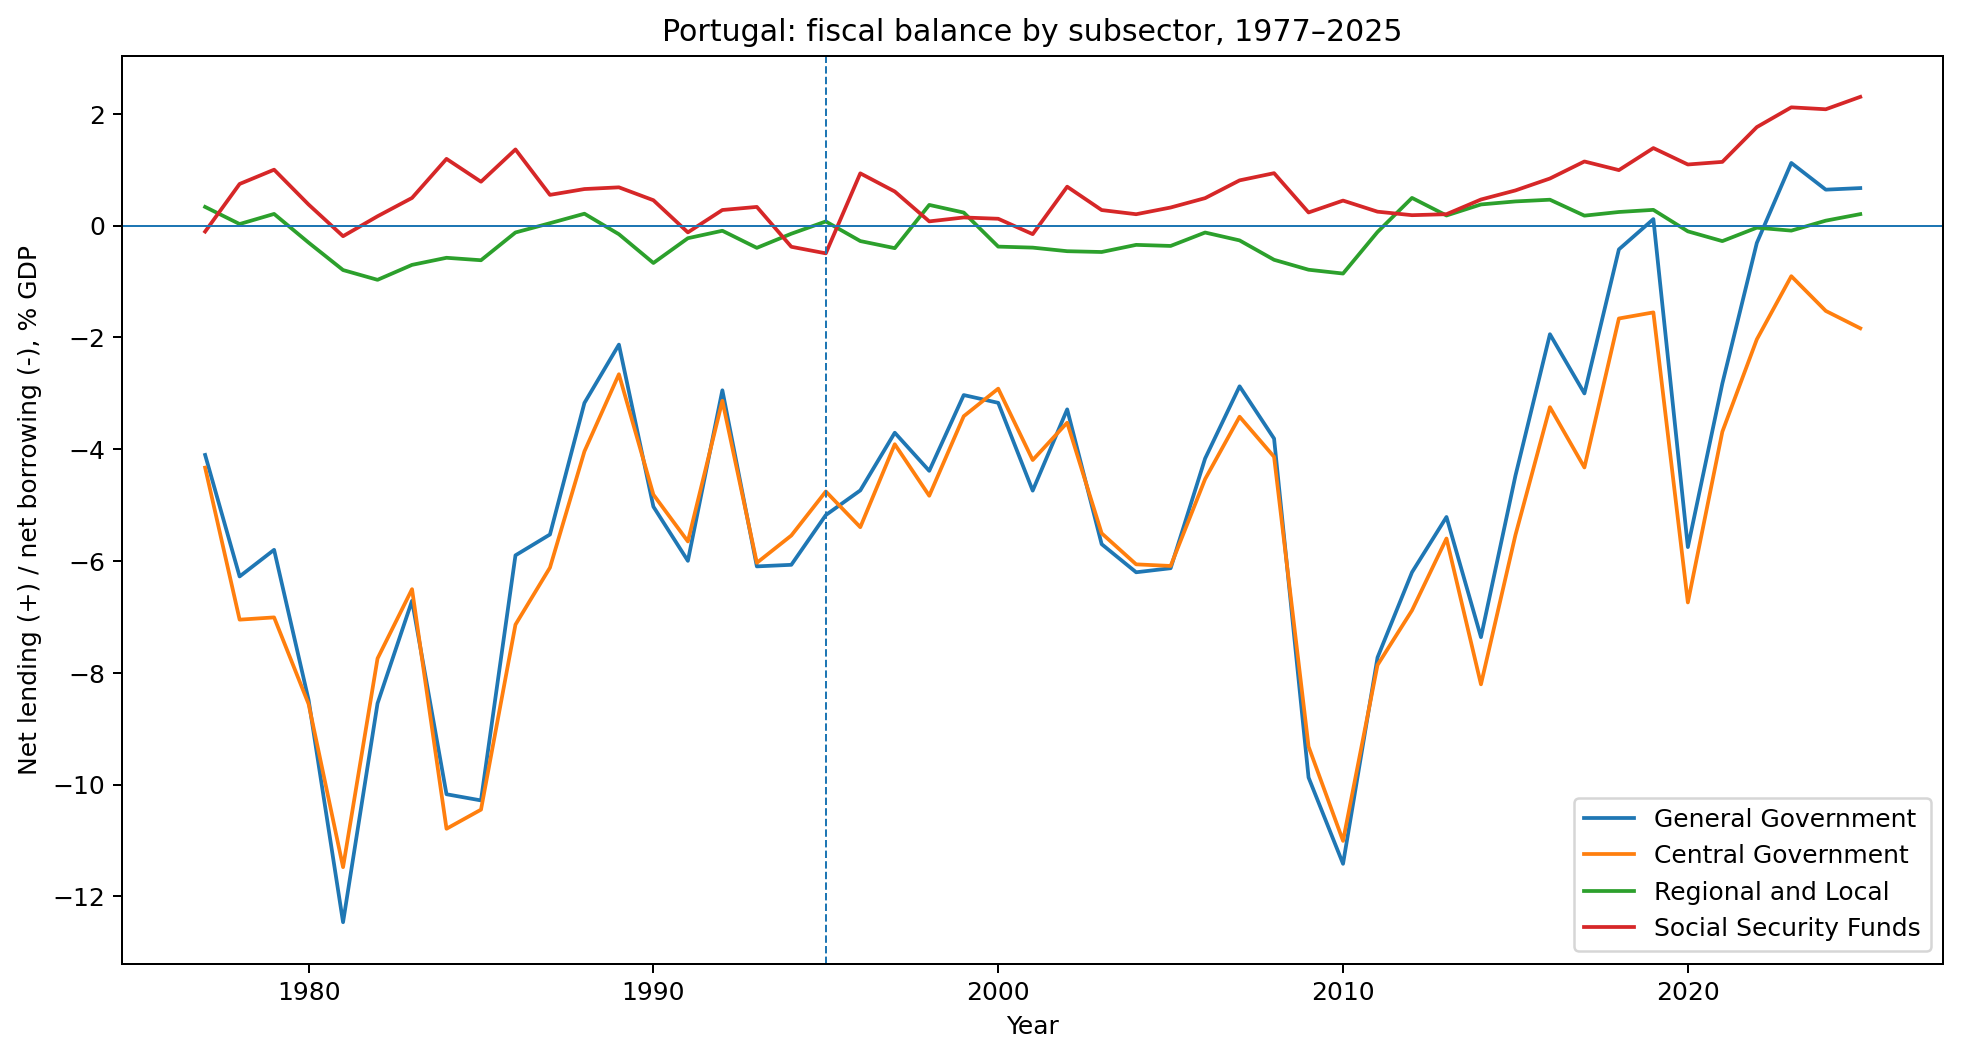
\includegraphics[width=\linewidth]{01_long_run_balances.png}
\caption{Net lending (+) and net borrowing (--) by subsector, \PanelStart--\PanelEnd,
as a percentage of nominal GDP. The vertical rule marks the 1995 source splice; the
series either side of it come from different source families and are not chained.
Sources: Banco de Portugal / INE long series and INE via PORDATA.}
\label{fig:longrun}
\end{figure}

That closeness is itself the first result. It says the aggregate balance has been
predominantly a Central Government quantity in level terms, which is what makes the
recent divergence at the right-hand edge of the figure notable rather than routine.

Figure~\ref{fig:contributions} draws the identity directly, stacking the signed
subsector contributions against the aggregate total. Where a tall stack sits under a
shallow line, the subsectors moved in opposite directions and offset one another.

\begin{figure}[htbp]
\centering
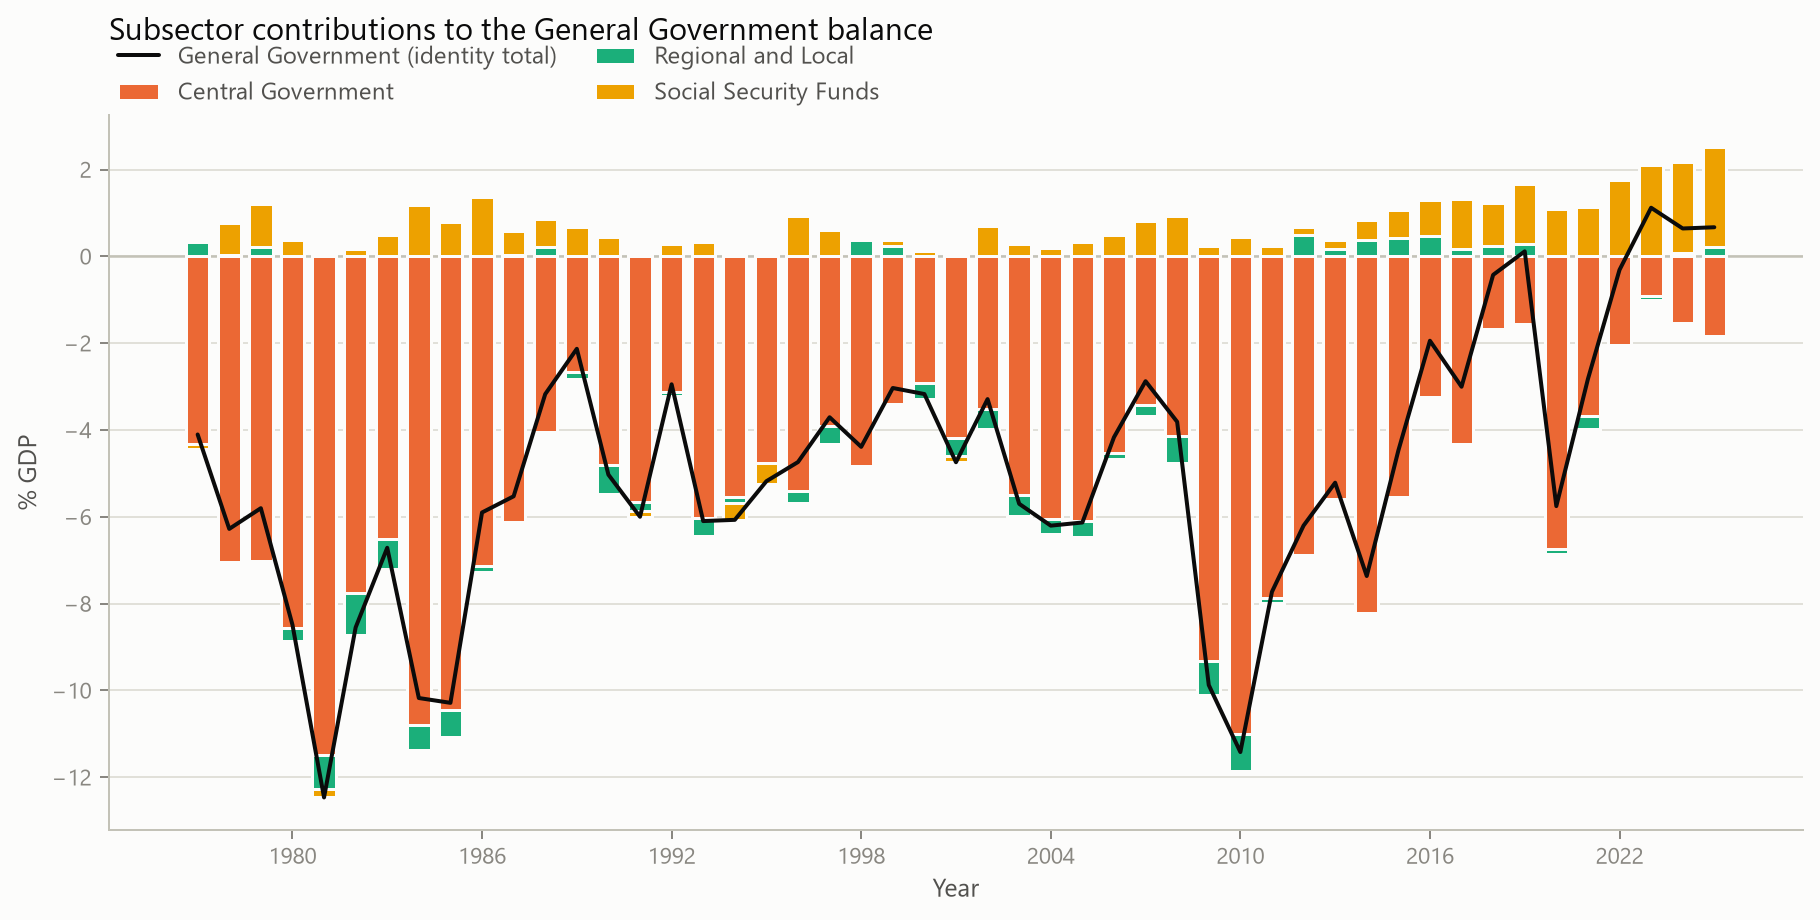
\includegraphics[width=\linewidth]{08_subsector_contributions.png}
\caption{The identity of Equation~\eqref{eq:identity} drawn: signed subsector
contributions stacked against the General Government total, as a percentage of GDP.
Positive and negative contributions stack away from zero independently, so the
visible column height equals the arithmetic sum of the layers.}
\label{fig:contributions}
\end{figure}

\subsection{Persistence, and why magnitudes are regime-specific}

Table~\ref{tab:composition} reports sign frequencies and magnitudes inside each
statistical regime.

\begin{table}[htbp]
\centering
\caption{Subsector composition of the general-government balance, by statistical regime. Magnitudes are reported inside each regime because the two differ enough that a pooled mean describes neither.}
\label{tab:composition}
\small
\fitwidth{%
\begin{tabular}{@{}llrrrrr@{}}
\toprule
Regime & Subsector & N & Positive & Negative & Mean (\% GDP) & Median (\% GDP) \\
\midrule
1977--1994 historical & General Government & 18 & 0 & 18 & -6.43 & -6.03 \\
1995--2025 modern & General Government & 31 & 4 & 27 & -4.04 & -4.17 \\
1977--1994 historical & Central Government & 18 & 0 & 18 & -6.61 & -6.31 \\
1995--2025 modern & Central Government & 31 & 0 & 31 & -4.67 & -4.33 \\
1977--1994 historical & Regional and Local & 18 & 5 & 13 & -0.27 & -0.19 \\
1995--2025 modern & Regional and Local & 31 & 13 & 18 & -0.09 & -0.10 \\
1977--1994 historical & Social Security Funds & 18 & 14 & 4 & 0.46 & 0.47 \\
1995--2025 modern & Social Security Funds & 31 & 29 & 2 & 0.72 & 0.61 \\
\bottomrule
\end{tabular}%
}
\end{table}


Three patterns are stable across both regimes. The Central Government balance is
negative in every observation of the panel, all \CentralNegativeYears\ of them. The
Social Security balance is positive in \SsfPositiveYears\ of \PanelYears, negative
in \SsfNegativeYears, with a longest unbroken positive run of
\SsfLongestPositiveRun\ years. Regional and Local Government is the only subsector
that changes sign with any regularity, positive in \RegionalPositiveYears\ years,
and it is small in both directions.

Magnitudes, by contrast, are strongly regime-dependent, and this is the reason the
table is split. The aggregate balance averages \GgMeanHistorical\% of GDP over
\PanelStart--1994 and \GgMeanModern\% over 1995--\PanelEnd. A pooled mean of
\GgMeanPooled\% falls between the two and corresponds to no period in the data.
Central Government moves from \CentralMeanHistorical\% to \CentralMeanModern\% and
the Social Security Funds from \SsfMeanHistorical\% to \SsfMeanModern\%.

Sign counts survive pooling far better than magnitudes, because a sign does not
depend on the level convention of a vintage. That asymmetry is why we pool the
counts in the discussion above and never pool the means.

\subsection{The years with a positive aggregate balance}

The aggregate balance is positive in \NumPositiveYears\ of \PanelYears\ years:
\PositiveYearList. Table~\ref{tab:positive} gives the composition of each.

\begin{table}[htbp]
\centering
\caption{Every year in which the aggregate balance is positive, with its subsector composition and the offset ratio.}
\label{tab:positive}
\small
\fitwidth{%
\begin{tabular}{@{}rrrrrrr@{}}
\toprule
Year & GG (M EUR) & Central (M EUR) & Regional/local (M EUR) & SSF (M EUR) & Non-SSF (M EUR) & Offset ratio \\
\midrule
2019 & 249 & -3,331 & 604 & 2,975 & -2,727 & 1.091 \\
2023 & 3,030 & -2,447 & -243 & 5,720 & -2,690 & 2.126 \\
2024 & 1,863 & -4,424 & 256 & 6,031 & -4,168 & 1.447 \\
2025 & 2,059 & -5,636 & 630 & 7,065 & -5,006 & 1.411 \\
\bottomrule
\end{tabular}%
}
\end{table}


The composition is the same in all \NumPositiveYears. The combined
non-Social-Security balance is negative, the Social Security balance is positive,
and the latter exceeds the former in absolute size --- which is precisely the
condition under which the offset ratio of Equation~\eqref{eq:offset} is defined and
exceeds one. In \LatestYear\ the identity reads
\[
\LatestGg = \LatestCentral + \LatestRegional + \LatestSsf \quad \text{M EUR},
\]
with a combined non-Social-Security balance of \LatestNonSsf\ million euro and an
offset ratio of \LatestOffset. In ratio terms the aggregate balance was
\LatestGgPct\% of GDP against a Social Security balance of \LatestSsfPct\%.

Figure~\ref{fig:offset} plots the ratio over the years in which it is defined.

\begin{figure}[htbp]
\centering
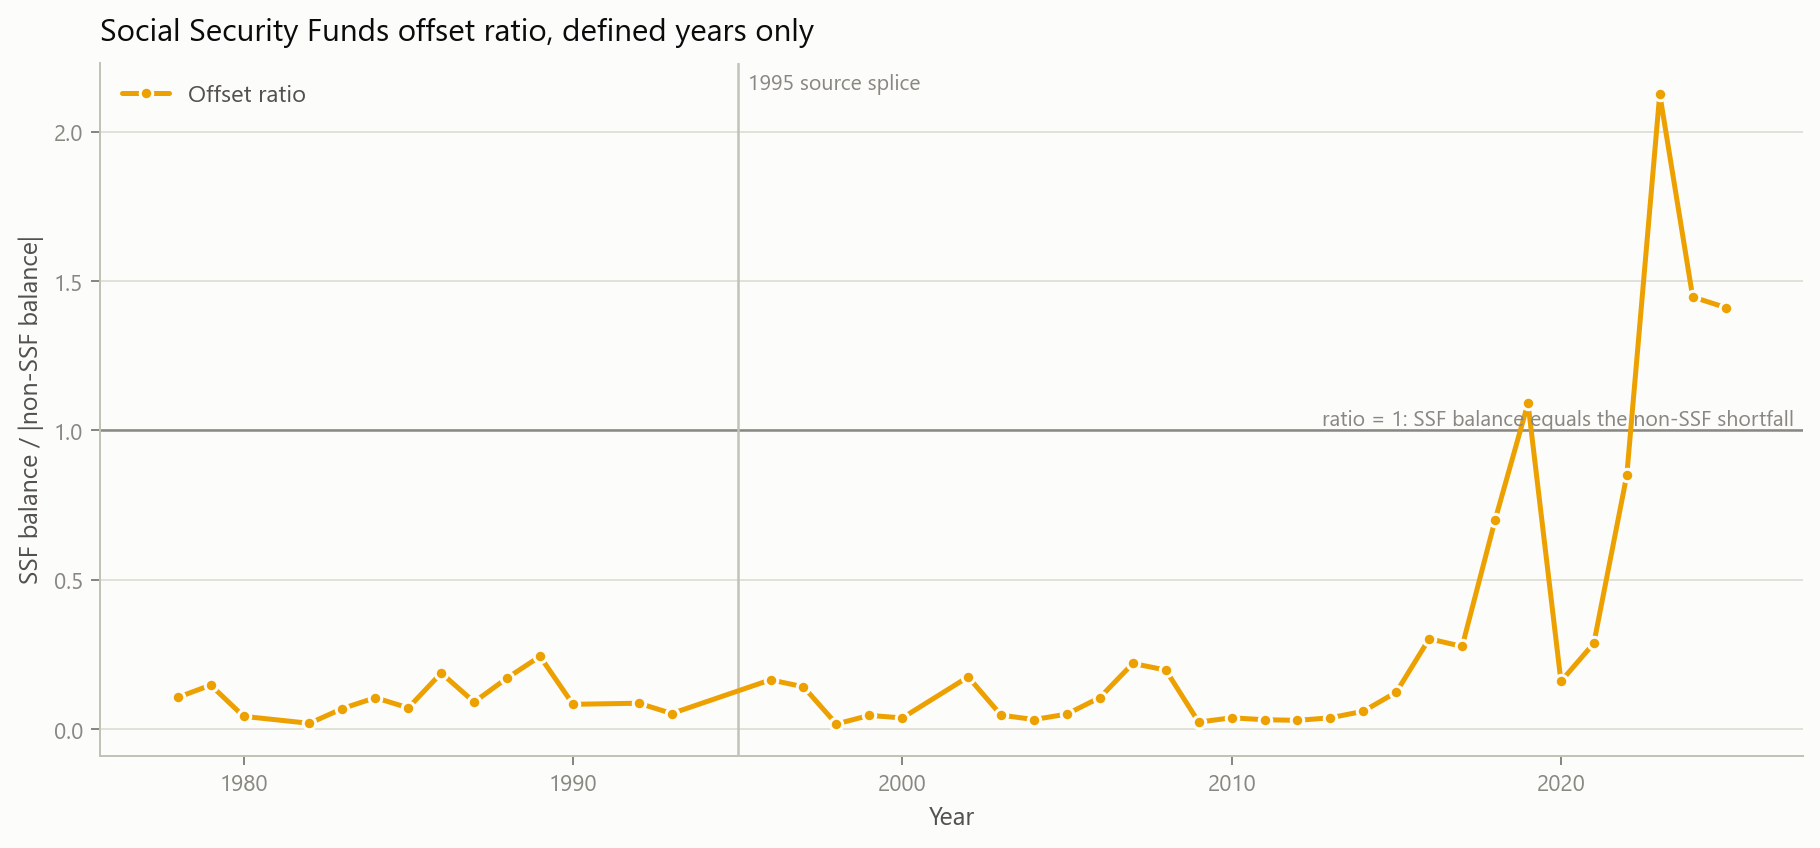
\includegraphics[width=\linewidth]{02_ssf_offset_ratio.png}
\caption{The offset ratio of Equation~\eqref{eq:offset}, for the years in which its
sign condition holds. The reference line at one marks the level at which the Social
Security balance equals the non-Social-Security shortfall. The ratio relates two
recorded quantities and is not a counterfactual.}
\label{fig:offset}
\end{figure}

We restate the caution of Section~\ref{sec:framework} because this is the result
most exposed to over-reading. That the ratio exceeds one in \LatestYear\ is a
statement about the relative size of two published numbers. It is not a statement
that the aggregate balance would have been negative under a different institutional
arrangement, and the identity contains nothing that could support such a statement.

\subsection{Annual movements}

Figures~\ref{fig:attributionmodern} and~\ref{fig:attributionhistorical} attribute
each annual change to the subsectors, on the GDP scaling of
Equation~\eqref{eq:scaled}. The two windows are drawn as separate panels and neither
crosses 1995: a single panel spanning the splice would place a vintage revision
among the economic movements and give it the same visual weight.

\begin{figure}[htbp]
\centering
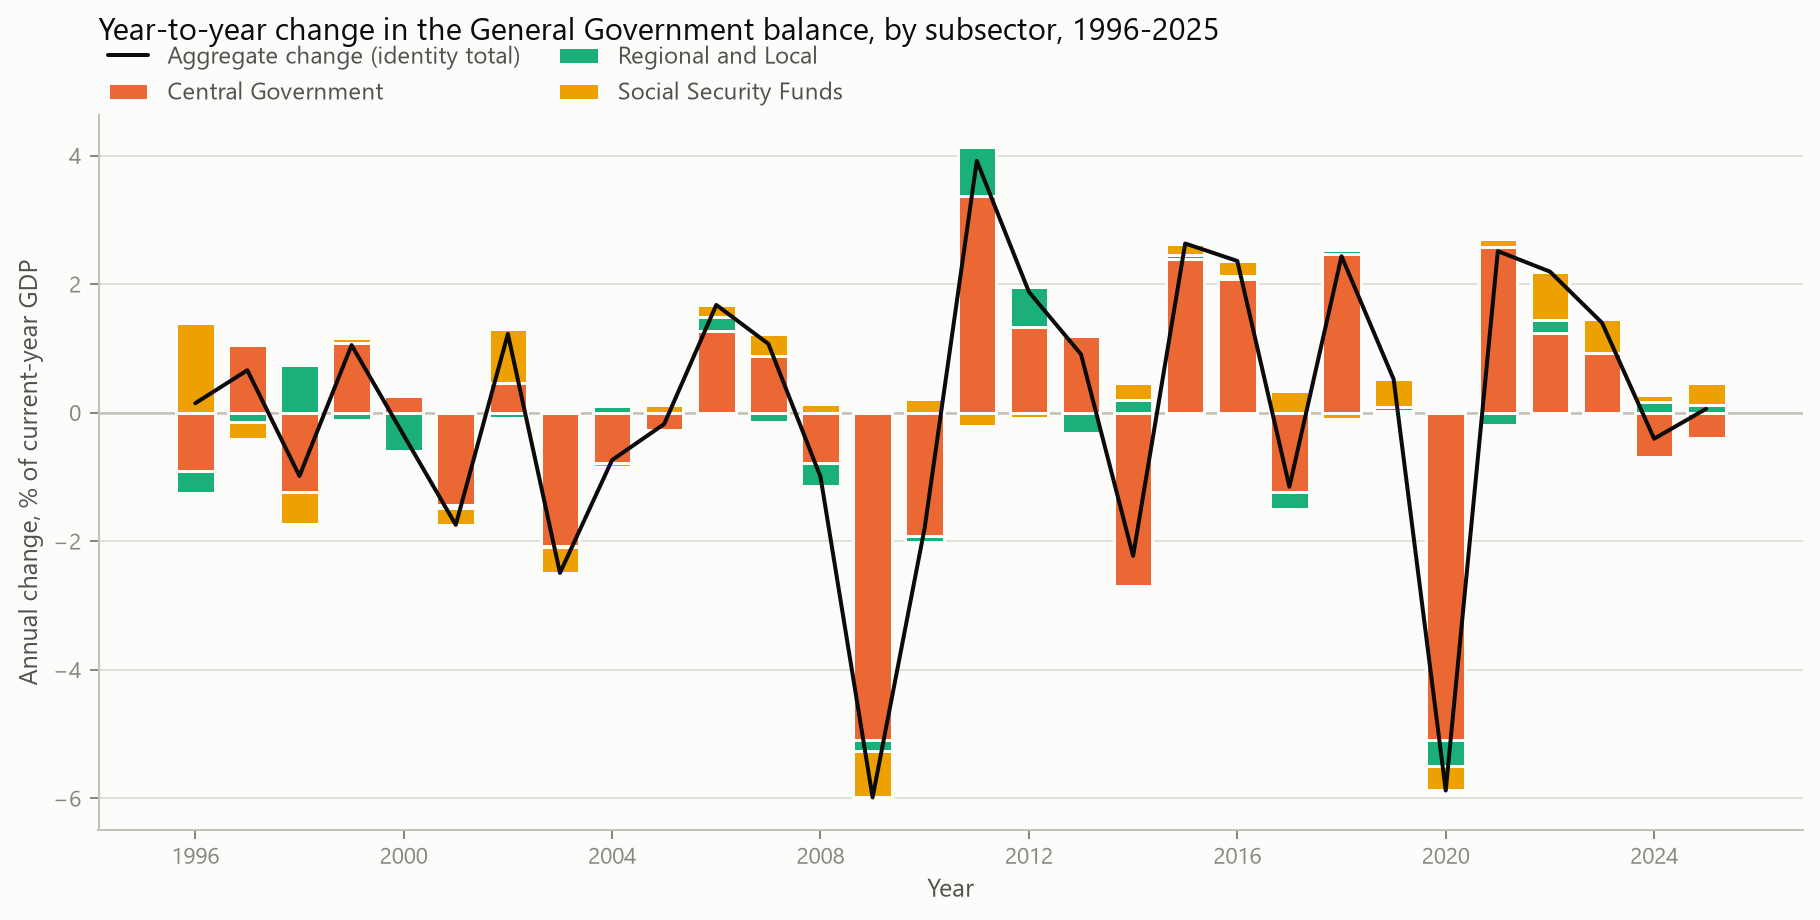
\includegraphics[width=\linewidth]{03_balance_change_attribution.png}
\caption{Annual change in the General Government balance attributed to subsectors,
1996--\PanelEnd, as a percentage of current-year GDP. The black line is the identity
total.}
\label{fig:attributionmodern}
\end{figure}

\begin{figure}[htbp]
\centering
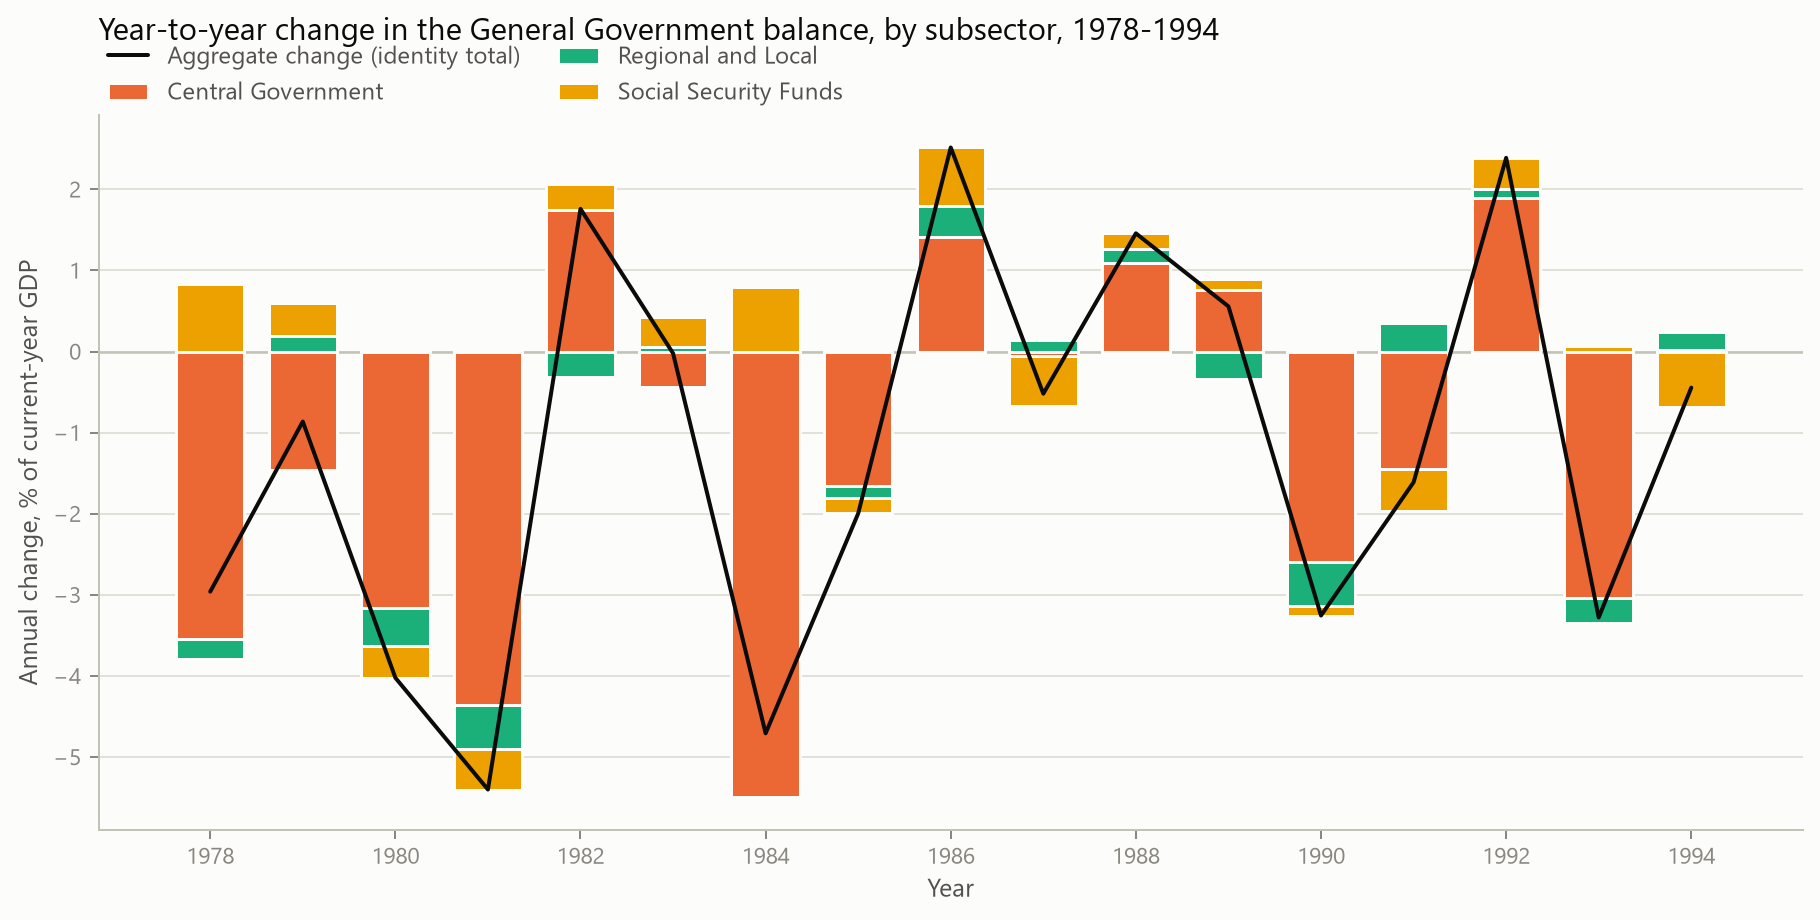
\includegraphics[width=\linewidth]{11_attribution_historical.png}
\caption{The same decomposition for 1978--1994, on the same scaling. The windows are
plotted separately because no change is computed through the 1995 splice.}
\label{fig:attributionhistorical}
\end{figure}

Table~\ref{tab:movements} ranks the \MovementsPerDirection\ largest improvements and
the \MovementsPerDirection\ largest deteriorations on that scaling, and attributes
each to a subsector and then to the revenue and expenditure movements behind it.

\begin{table}[htbp]
\centering
\caption{The largest annual improvements and deteriorations, ranked on the change scaled by current-year GDP, with the subsector and the revenue or expenditure movements that composed each one.}
\label{tab:movements}
\small
\fitwidth{%
\begin{tabular}{@{}lrrrrrrr@{}}
\toprule
Direction & Year & Change (\% GDP) & Central (M EUR) & Regional/local (M EUR) & SSF (M EUR) & From revenue (M EUR) & From expenditure (M EUR) \\
\midrule
Improvement & 2011 & 3.92 & 5,937 & 1,342 & -366 & 1,796 & -5,117 \\
Improvement & 2015 & 2.63 & 4,283 & 121 & 321 & 1,854 & -2,871 \\
Improvement & 2021 & 2.52 & 5,570 & -394 & 270 & 9,188 & 3,742 \\
Improvement & 1986 & 2.52 & 355 & 97 & 181 & 2,092 & 1,458 \\
Improvement & 2018 & 2.44 & 5,053 & 151 & -208 & 4,794 & -203 \\
Deterioration & 2009 & -5.98 & -8,939 & -289 & -1,268 & -3,802 & 6,694 \\
Deterioration & 2020 & -5.88 & -10,224 & -811 & -777 & -4,176 & 7,636 \\
Deterioration & 1981 & -5.40 & -385 & -48 & -45 & 573 & 1,051 \\
Deterioration & 1984 & -4.71 & -922 & -1 & 133 & 943 & 1,733 \\
Deterioration & 1980 & -4.02 & -233 & -34 & -29 & 523 & 819 \\
\bottomrule
\end{tabular}%
}
\par\smallskip
\begin{minipage}{\linewidth}\footnotesize\itshape 1995 is excluded: the 1994-to-1995 change straddles the vintage splice in both panels and mixes a statistical revision with an economic movement.\end{minipage}
\end{table}


The scaling changes what the ranking shows, which is the point of using it.
\HistoricalEpisodes\ of the ten episodes fall in the historical regime --- episodes
that a nominal ranking places nowhere near the top, because the euro amounts
involved are small relative to modern GDP. The largest single improvement is
\TopImprovementYear\ at \TopImprovementPct\ percentage points of GDP and the largest
deterioration is \TopDeteriorationYear\ at \TopDeteriorationPct.

Central Government accounts for the largest share of every one of the ten episodes.
Given that it also carries the level of the aggregate balance
(Section~\ref{sec:results}), this is less surprising than it first appears, and it
is worth stating what it does not mean: the subsector accounting arithmetically for
a movement has not been shown to have produced it.

\subsection{Social Security mechanisms}

We now turn to the second research question. Two distinct layers have to be kept
apart, and the value of the exercise lies in the separation.

\paragraph{The national-accounts layer.} The ESA 2010 Social Security Funds sector
is the entity that appears in Equation~\eqref{eq:identity}. In \LatestYear\ social
contributions were \ContributionSharePct\% of its total revenue.
Figure~\ref{fig:ssfshare} plots that share over the panel.

\begin{figure}[htbp]
\centering
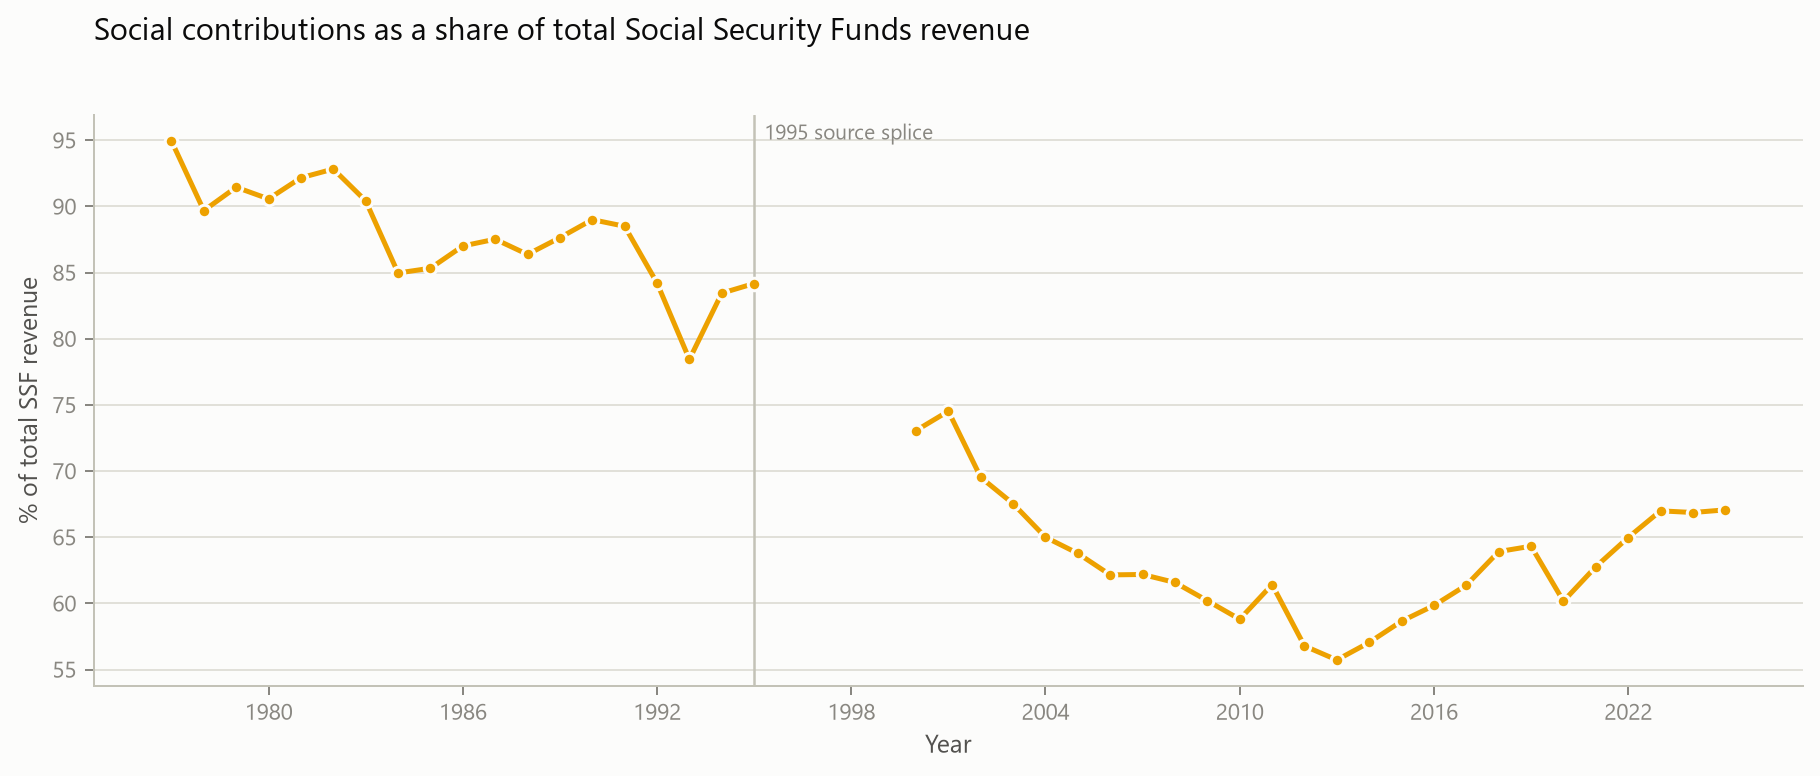
\includegraphics[width=\linewidth]{05_ssf_contribution_share.png}
\caption{Social contributions as a share of total Social Security Funds revenue.
The line breaks at 1996--1999, where subsector components do not exist in either
source family.}
\label{fig:ssfshare}
\end{figure}

\paragraph{The budget-execution layer.} The CFP publishes the system decomposed into
the Previdential system, the Social Protection of Citizenship system and special
regimes. These are budget-execution aggregates on a different accounting boundary.
Figure~\ref{fig:ssfsystems} shows them.

\begin{figure}[htbp]
\centering
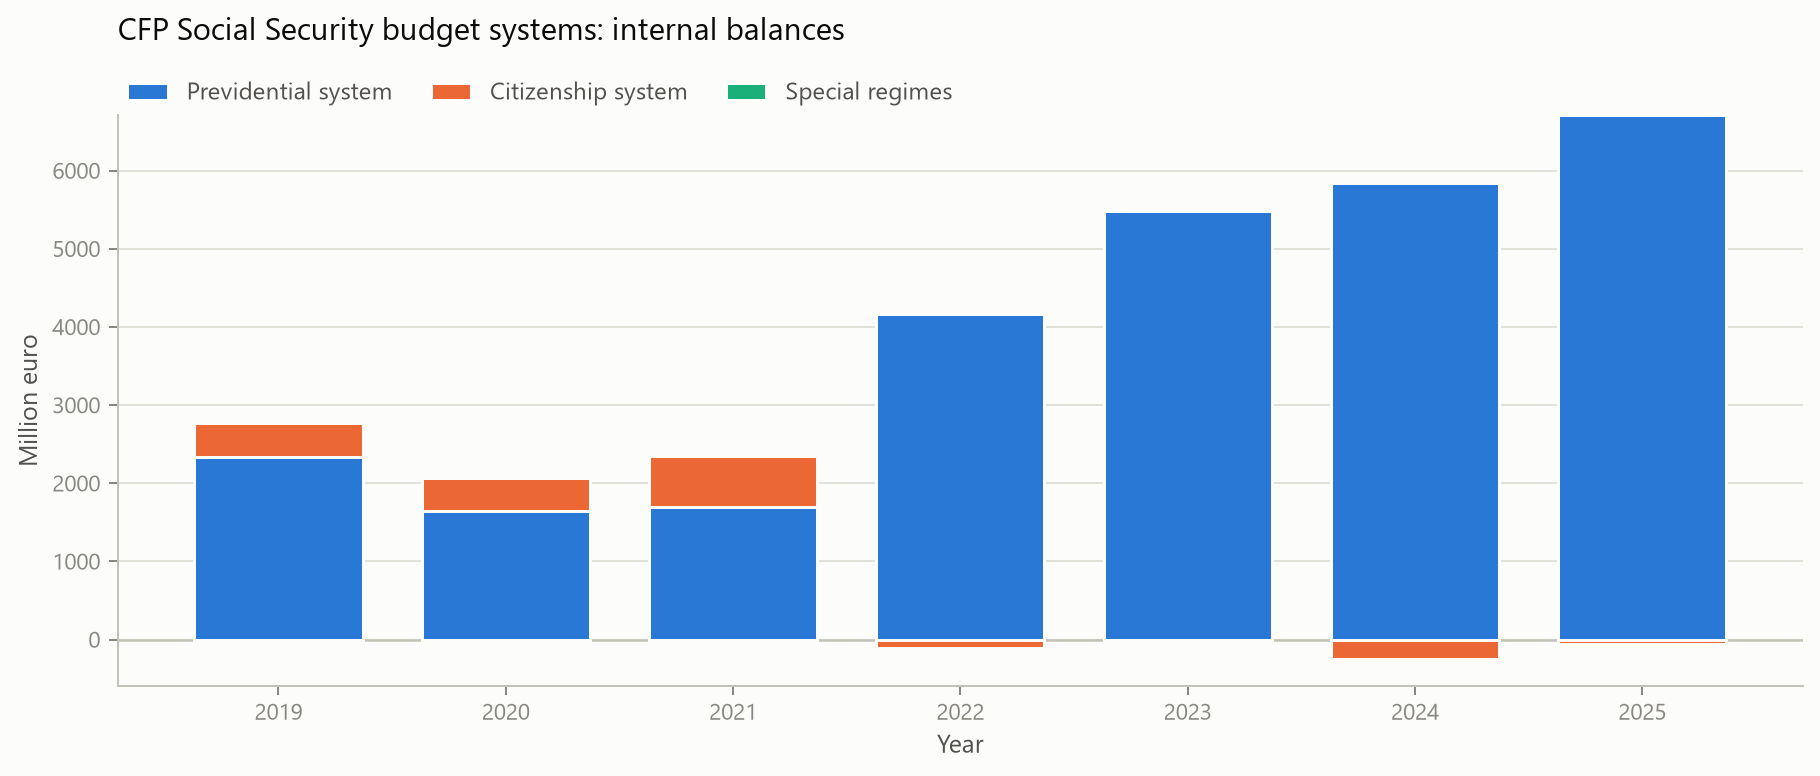
\includegraphics[width=\linewidth]{13_ssf_budget_systems.png}
\caption{CFP internal Social Security balances by system, in million euro. The
movement over the published window is concentrated in the Previdential system.}
\label{fig:ssfsystems}
\end{figure}

The movement is concentrated in one system. The Previdential balance goes from
\PrevidentialFirst\ million euro in \PrevidentialFirstYear\ to
\PrevidentialLatest\ million in \LatestYear, while the Citizenship balance stays
small in both directions, standing at \CitizenshipLatest\ million in \LatestYear.
Since contributions are the dominant revenue item of the Previdential system, and
since the contribution share of national-accounts revenue rose over the same years,
the two layers are telling a consistent story about where the movement sits. Neither
identifies why it happened, and we do not speculate: a contributory balance moves
with employment, wages, contribution rates, entitlement rules and demographics
simultaneously, and separating them needs a model this paper does not build.

\paragraph{Why the two layers must not be interchanged.} This is a methodological
result, and it is the one we would most want a reader to carry away.
Table~\ref{tab:ssfboundary} places the two side by side.

\begin{table}[htbp]
\centering
\caption{Two accounting boundaries for Social Security, reported side by side. The columns are never added, netted or reconciled.}
\label{tab:ssfboundary}
\small
\fitwidth{%
\begin{tabular}{@{}rrrrrr@{}}
\toprule
Year & ESA 2010 (M EUR) & Budget systems (M EUR) & Previdential (M EUR) & Citizenship (M EUR) & Difference (M EUR) \\
\midrule
2019 & 2,975 & 2,776 & 2,333 & 443 & 199 \\
2020 & 2,198 & 2,072 & 1,649 & 423 & 126 \\
2021 & 2,468 & 2,348 & 1,695 & 653 & 120 \\
2022 & 4,299 & 4,062 & 4,172 & -110 & 237 \\
2023 & 5,720 & 5,486 & 5,485 & 1 & 234 \\
2024 & 6,031 & 5,595 & 5,840 & -245 & 436 \\
2025 & 7,065 & 6,657 & 6,712 & -55 & 408 \\
\bottomrule
\end{tabular}%
}
\end{table}


In \LatestYear\ the ESA 2010 balance was \SsfEsaLatest\ million euro while the three
budget systems summed to \SsfBudgetLatest\ million, a difference of
\SsfBoundaryLatest\ million. Across the \SsfBoundaryYears\ overlapping years the
difference ranges from \SsfBoundaryMin\ to \SsfBoundaryMax\ million euro. It is
never zero.

Figure~\ref{fig:ssfboundary} makes the scale problem visible: on a shared axis the
two series are nearly identical, and the difference is only legible on an axis of
its own.

\begin{figure}[htbp]
\centering
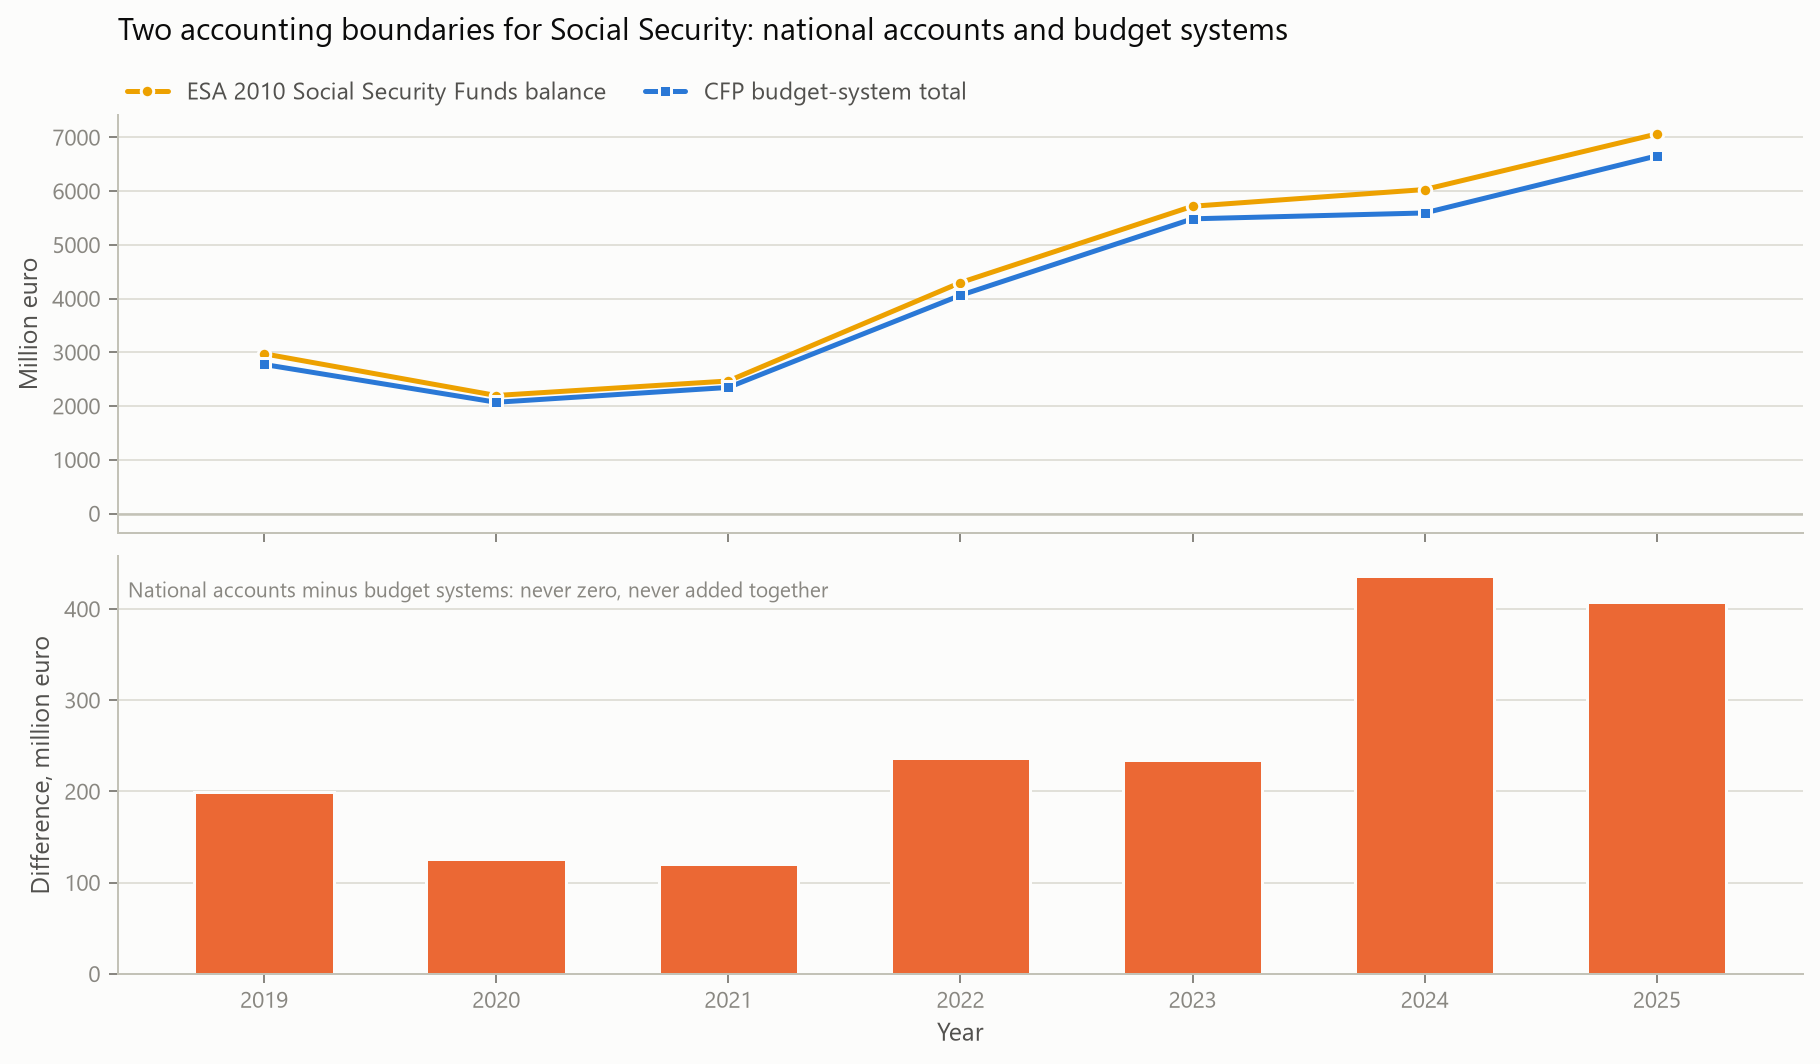
\includegraphics[width=\linewidth]{14_ssf_accounting_boundary.png}
\caption{The two Social Security accounting boundaries. Upper panel: both balances
on a shared axis, where they are almost indistinguishable. Lower panel: the
difference on its own axis. The two are never added, netted or reconciled here.}
\label{fig:ssfboundary}
\end{figure}

The consequence is practical. A Social Security figure quoted from the budget
documents is not the figure that enters the national-accounts identity, and
substituting one for the other introduces an error of a few hundred million euro
without any signal that it has happened. We therefore report both and add neither.

\subsection{Primary balance: the headline sign is not the underlying sign}

The Central Government balance is negative in all \CentralNegativeYears\ years of
the panel. Read alone, that invites a strong conclusion: that the subsector runs an
underlying deficit throughout. The detailed accounts do not support it.

The primary balance is reconstructed as $PB_{i,t} = B_{i,t} + I_{i,t}$, where $I$ is
interest expenditure, and checked against the published primary-balance row.
Table~\ref{tab:primarysigns} contrasts the two sign frequencies.

\begin{table}[htbp]
\centering
\caption{Headline against primary balance sign frequencies, over the sector-years for which interest expenditure is published.}
\label{tab:primarysigns}
\small
\fitwidth{%
\begin{tabular}{@{}lrrrrr@{}}
\toprule
Subsector & N & Headline $<0$ & Primary $>0$ & Mean interest (\% GDP) & Peak interest (\% GDP) \\
\midrule
General Government & 49 & 45 & 22 & 4.16 & 7.89 \\
Central Government & 45 & 45 & 15 & 4.17 & 7.73 \\
Regional and Local & 45 & 29 & 20 & 0.13 & 0.62 \\
Social Security Funds & 45 & 6 & 39 & 0.00 & 0.04 \\
\bottomrule
\end{tabular}%
}
\end{table}


Over the \PrimaryObservedYears\ years for which interest expenditure is published,
the Central Government headline balance is negative in
\PrimaryHeadlineNegative\ --- all of them --- while the primary balance is positive
in \PrimaryPositiveYears: \PrimaryPositiveList. Those years are not confined to the
recent period; they run from \PrimaryPositiveFirst\ to \PrimaryPositiveLast. Interest
averaged \InterestMeanPct\% of GDP over the panel and peaked at
\InterestPeakPct\%, and that is the arithmetic separating the two series.
Figure~\ref{fig:primary} shows the primary balance crossing zero repeatedly while the
headline balance never does.

\begin{figure}[htbp]
\centering
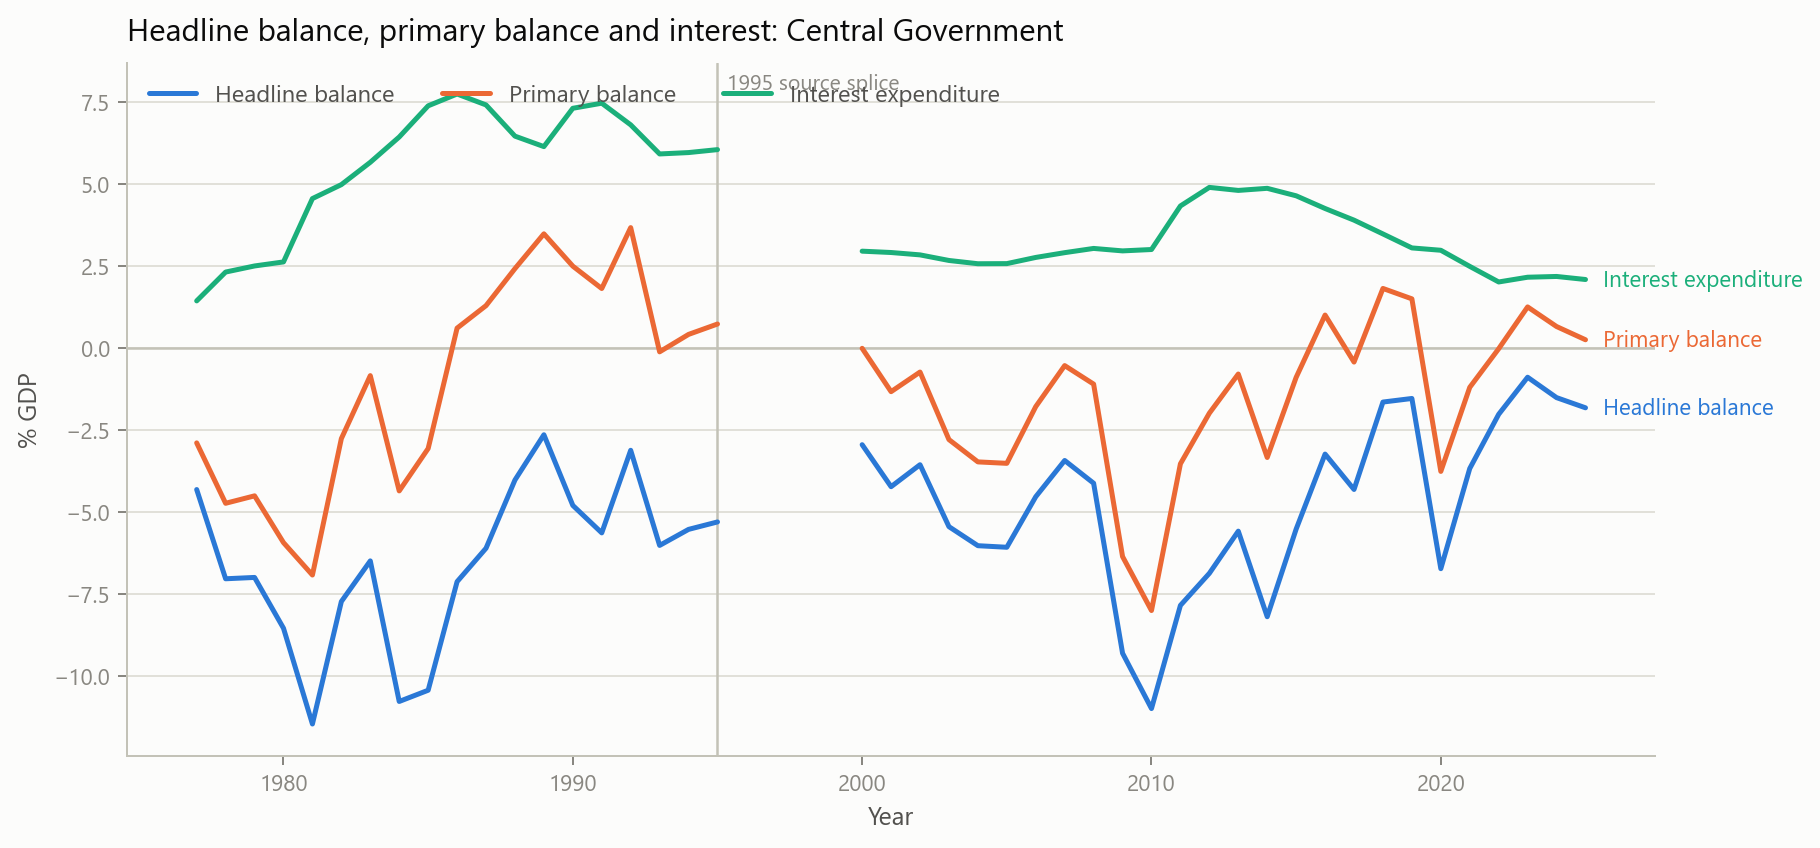
\includegraphics[width=\linewidth]{06_central_primary_balance.png}
\caption{Central Government headline balance, primary balance and interest
expenditure, as shares of GDP. The primary balance crosses zero repeatedly; the
headline balance does not. The line breaks at 1996--1999.}
\label{fig:primary}
\end{figure}

Both statements are descriptive and they do not conflict. The correct summary is
that the Central Government B.9 is negative throughout the panel \emph{and} that its
primary balance is positive in a non-trivial minority of the observed years.

The symmetric caution applies. A positive primary balance is not a sustainability
result: it excludes interest by construction and therefore says nothing about the
debt path, which depends on the interest burden it removes. Neither series, on its
own, licenses a conclusion about sustainability.

% Authored. Tables and numbers come from generated/.

\section{Robustness and Accounting Boundaries}
\label{sec:robustness}

\subsection{The 1995 splice}

The splice is the single largest threat to the level results, and it is handled by
restriction rather than by adjustment. Both 1995 vintages are retained; the revision
between them is non-zero for every subsector; no level statistic is averaged across
the boundary; and no annual change is computed through it. The regime split of
Table~\ref{tab:composition} is the form in which magnitudes are reported precisely
because a pooled magnitude would embed the splice silently.

Sign-based results are less exposed to the splice than magnitudes, and
Section~\ref{sec:data} checks that rather than asserting it: sign classifications are
unchanged across both source overlaps this panel retains. The persistence results of
Section~\ref{sec:results} therefore carry more weight than the means beside them, and
we have kept the two visually separate for that reason.

\subsection{How firm are the change-point dates?}

The piecewise-constant mean model of Section~\ref{sec:method} selects break dates,
and a selected date reads as more determined than it is --- particularly here, where
the penalised criterion follows \citet{yao1988} in form but is one of several the
change-point literature admits \citep{baiperron1998}. Two guards are reported.

The first is a BIC margin over the next-best break count, which says how decisively
the selection beat its alternatives. The second is a sensitivity grid: detection
re-run over \BreakSpecifications\ combinations of the two tuning parameters, neither
of which is estimated from the data. A date that survives only one combination is a
property of that choice rather than of the series.

Table~\ref{tab:breakstability} reports the grid summary, and
Appendix~\ref{sec:changepoints} the full detail.

\begin{table}[htbp]
\centering
\caption{Sensitivity of the detected mean shifts to the two tuning choices, over twelve specifications per series.}
\label{tab:breakstability}
\small
\fitwidth{%
\begin{tabular}{@{}llrlrr@{}}
\toprule
Regime & Subsector & Modal breaks & Modal dates & Share at modal dates & Distinct date sets \\
\midrule
1977--1994 historical & General Government & 1 & 1986 & 0.83 & 2 \\
1995--2025 modern & General Government & 2 & 2009, 2015 & 0.42 & 4 \\
1977--1994 historical & Central Government & 1 & 1987 & 1.00 & 1 \\
1995--2025 modern & Central Government & 2 & 2009, 2016 & 0.67 & 2 \\
1977--1994 historical & Regional and Local & 0 & -- & 0.83 & 2 \\
1995--2025 modern & Regional and Local & 2 & 2012 & 0.33 & 6 \\
1977--1994 historical & Social Security Funds & 0 & -- & 1.00 & 1 \\
1995--2025 modern & Social Security Funds & 1 & 2017 & 0.67 & 3 \\
\bottomrule
\end{tabular}%
}
\end{table}


The grid is not a formality: it changes what may be claimed. In
\BreakModalAgree\ of the \BreakSeries\ series the preferred specification returns the
modal set of dates. In the remaining series it does not, and for those the selected
dates follow the tuning choice. The least stable case is
\WeakestBreakSector\ in the modern regime, where the modal dates hold in only
\WeakestBreakShare\% of the grid across \WeakestBreakSets\ distinct date sets.

Accordingly we describe every date as a candidate rather than a finding, and no
break year should be quoted from this paper without its share. We also attach no
historical cause to any of them, and note that a five-year minimum segment means a
shift in the last four years of the sample cannot be detected at all.

\subsection{Intergovernmental transfers and the location of a balance}

Because the subsectors are consolidated, a transfer between them changes the
components and not the aggregate. This makes the \emph{location} of a balance within
general government partly a function of the transfer convention, which matters for
interpreting composition results.

The historical source tables identify current and capital transfers between public
administrations, which supports a purely mechanical sensitivity for
\PanelStart--1995:
\[
B^{sens}_{i,t} = B_{i,t} - \left(T^{received}_{i,t} - T^{paid}_{i,t}\right).
\]

We compute it and deliberately decline to label it an underlying or true balance,
and we never use it to restate B.9. The reason is substantive rather than cautious:
a transfer normally finances an expenditure responsibility assigned to the
recipient, so removing the transfer while leaving the responsibility in place does
not describe a coherent alternative arrangement. Which transfer discharges which
statutory obligation is a legal question, not an accounting one. What the
sensitivity quantifies is how much the recorded location of a balance depends on the
convention --- and it is reported for that purpose only.

The same reasoning is why no Social Security balance in this paper has State
transfers netted out of it.

\subsection{What the balance does not determine}

Two limits on the reach of these results are worth stating explicitly, because both
concern inferences a reader may reasonably be tempted to draw.

The balance does not determine the debt path. The change in debt equals minus the
balance plus a stock-flow adjustment that absorbs financial-asset transactions,
valuation effects and timing differences, and in several years in these data the
adjustment is the larger of the two terms. Whether such residuals reflect accounting
responses to fiscal rules \citep{vonhagen2006} or are smaller and less systematic
than that literature suggested \citep{seiferling2013} is a live question on which we
take no position. Its relevance here is narrower: a composition result about
balances is not a result about debt.

The balance does not identify a mechanism. The decompositions of
Section~\ref{sec:method} locate a movement in the accounts; they do not explain it.
Nothing here separates cyclical from discretionary movements, and no cyclical
adjustment is attempted. A specification relating balances to nominal GDP growth exists
in the repository and is reported there with its weaknesses set out. It supports no claim
in this paper, because its dependent variable and its regressor share a construction
through nominal GDP and its fits are very low --- \GdpRSquaredLow\ to
\GdpRSquaredHigh\ across \GdpRSquaredSeries\ series. It appears here for one purpose
only, as the point of comparison in Section~\ref{sec:contributionbase}: quoting its fit
to say that a better-specified regressor does better is a use of the number that its
weaknesses do not undermine.

For the Social Security side specifically, that gap can be narrowed rather than left open.
Equation~\eqref{eq:ssfchange} shows that contributions are the dominant positive term in
the recent balance changes, and the Council attributes the contribution growth to rising
employment and average earnings \citep{cfp_ss_outturn2025}.
Section~\ref{sec:contributionbase} models the contribution base directly, relating the
change in contributions to the change in the aggregate wage bill $W_t = N_t \bar{w}_t$
rather than to aggregate nominal growth. The regressor there is the largest observable
reference base for the levy, and at \WageBillRSquared\ the fit is several times tighter
than anything the specification criticised here achieves.

% Authored. Tables and numbers come from generated/.

\section{The Contribution Base}
\label{sec:contributionbase}

Every Social Security result to this point is internal to the fiscal accounts.
Section~\ref{sec:results} establishes that contributions are the largest positive term
in the recent balance changes, and stops there: an accounting location, not an economic
mechanism. This section supplies the link to something outside the accounts.

\subsection{The base and the ratio}

Contributions are levied on wages, so the natural base is the aggregate wage bill of the
economy, $W_t = N_t \bar{w}_t$, with $N$ employees and $\bar{w}$ the average wage per
employee. Writing the contributions-to-wage-bill ratio as $\tau_t = C_t / W_t$, the
change in contributions decomposes exactly:
\begin{equation}
\Delta C_t = \underbrace{\tau_{t-1} \Delta W_t}_{\text{wage-bill component}}
+ \underbrace{W_{t-1} \Delta \tau_t}_{\text{ratio component}}
+ \underbrace{\Delta W_t \Delta \tau_t}_{\text{interaction}}.
\label{eq:contributionbase}
\end{equation}
The wage-bill component splits again by the same identity, into an employment component
and an average-wage component. Both decompositions are exact. The interaction term is
carried rather than dropped or shared between the factors, because either would make the
decomposition inexact while looking tidier.

We call $\tau$ a ratio and never a rate, deliberately. ``Rate effect'' would invite the
reading that a movement in $\tau$ reflects a change in the statutory levy, and the next
paragraph explains why that reading would be wrong.

The wage bill and the employee count are the Portuguese national accounts compiled by
Statistics Portugal, taken from the harmonised dissemination of those accounts
\citep{ine_wage_bill,ine_employment}. We use wages and salaries (D.11) rather than
compensation of employees (D.1), because D.1 already includes employers' social
contributions and would place part of the numerator inside the denominator.

\paragraph{What $\tau$ is not.} It is not a statutory contribution rate.
National-accounts social contributions received by the Social Security Funds include
imputed contributions and contributions on bases other than employee wages, notably the
self-employed. It is a ratio between two published aggregates, and it moves with
coverage, compliance and composition as well as with legislated rates. It stands at
\EffectiveRateLatest\ in \BaseYear\ against a panel mean of \EffectiveRateMean, both
well below the headline levy, which is itself a sign that the two are not the same
object.

\subsection{What moved contributions}

\begin{table}[htbp]
\centering
\caption{The annual change in Social Security contributions, split into the movement of the wage bill and the movement of the effective ratio, and the wage bill split again into employment and average wages.}
\label{tab:contributionbase}
\small
\fitwidth{%
\begin{tabular}{@{}rrrrrrr@{}}
\toprule
Year & $\Delta$ contributions & From wage bill & From rate & $\Delta$ wage bill & From employment & From average wage \\
\midrule
2018 & 1,166 & 947 & 206 & 3,998 & 1,423 & 2,521 \\
2019 & 1,484 & 1,014 & 443 & 4,225 & 478 & 3,722 \\
2020 & 311 & 28 & 283 & 116 & -1,400 & 1,544 \\
2021 & 1,430 & 1,268 & 152 & 5,071 & 852 & 4,172 \\
2022 & 2,289 & 2,110 & 163 & 8,372 & 2,985 & 5,194 \\
2023 & 2,806 & 2,685 & 107 & 10,572 & 2,000 & 8,383 \\
2024 & 2,557 & 2,056 & 463 & 8,058 & 992 & 6,996 \\
2025 & 2,468 & 1,870 & 560 & 7,196 & 2,253 & 4,842 \\
\bottomrule
\end{tabular}%
}
\par\smallskip
\begin{minipage}{\linewidth}\footnotesize\itshape The interaction terms are carried rather than dropped or shared between the factors, because either would make the decomposition inexact.\end{minipage}
\end{table}


In \BaseYear\ contributions rose by \BaseContributionsChange\ million euro, which
decomposes as
\[
\BaseContributionsChange = \underbrace{\BaseFromWageBill}_{\text{wage bill}}
+ \underbrace{\BaseFromRate}_{\text{ratio}}
+ \underbrace{\BaseRatioInteraction}_{\text{interaction}}.
\]
The wage bill did most of the work, but not all of it. The wage bill itself rose by
\BaseWageBillChange\ million, and that splits the same way:
\[
\BaseWageBillChange = \underbrace{\BaseFromEmployment}_{\text{employees}}
+ \underbrace{\BaseFromAverageWage}_{\text{average wage}}
+ \underbrace{\BaseWageInteraction}_{\text{interaction}}.
\]
The interaction terms are small here, but they are stated rather than absorbed: a paper
that insists the decomposition is exact should not present a two-term version of a
three-term identity.

Figure~\ref{fig:contributionbase} shows both decompositions over the modern period, and
the two crises are where the mechanism is clearest. In the austerity years the wage bill
contracts on both margins at once, employment and wages falling together. In 2020 the
two margins move in opposite directions --- employment falls while average wages rise ---
so the wage bill is almost flat and contributions rise anyway, on the ratio rather than
the base. Recent years are the reverse of austerity: the base grows strongly, and average
wages contribute more than employment.

\begin{figure}[htbp]
\centering
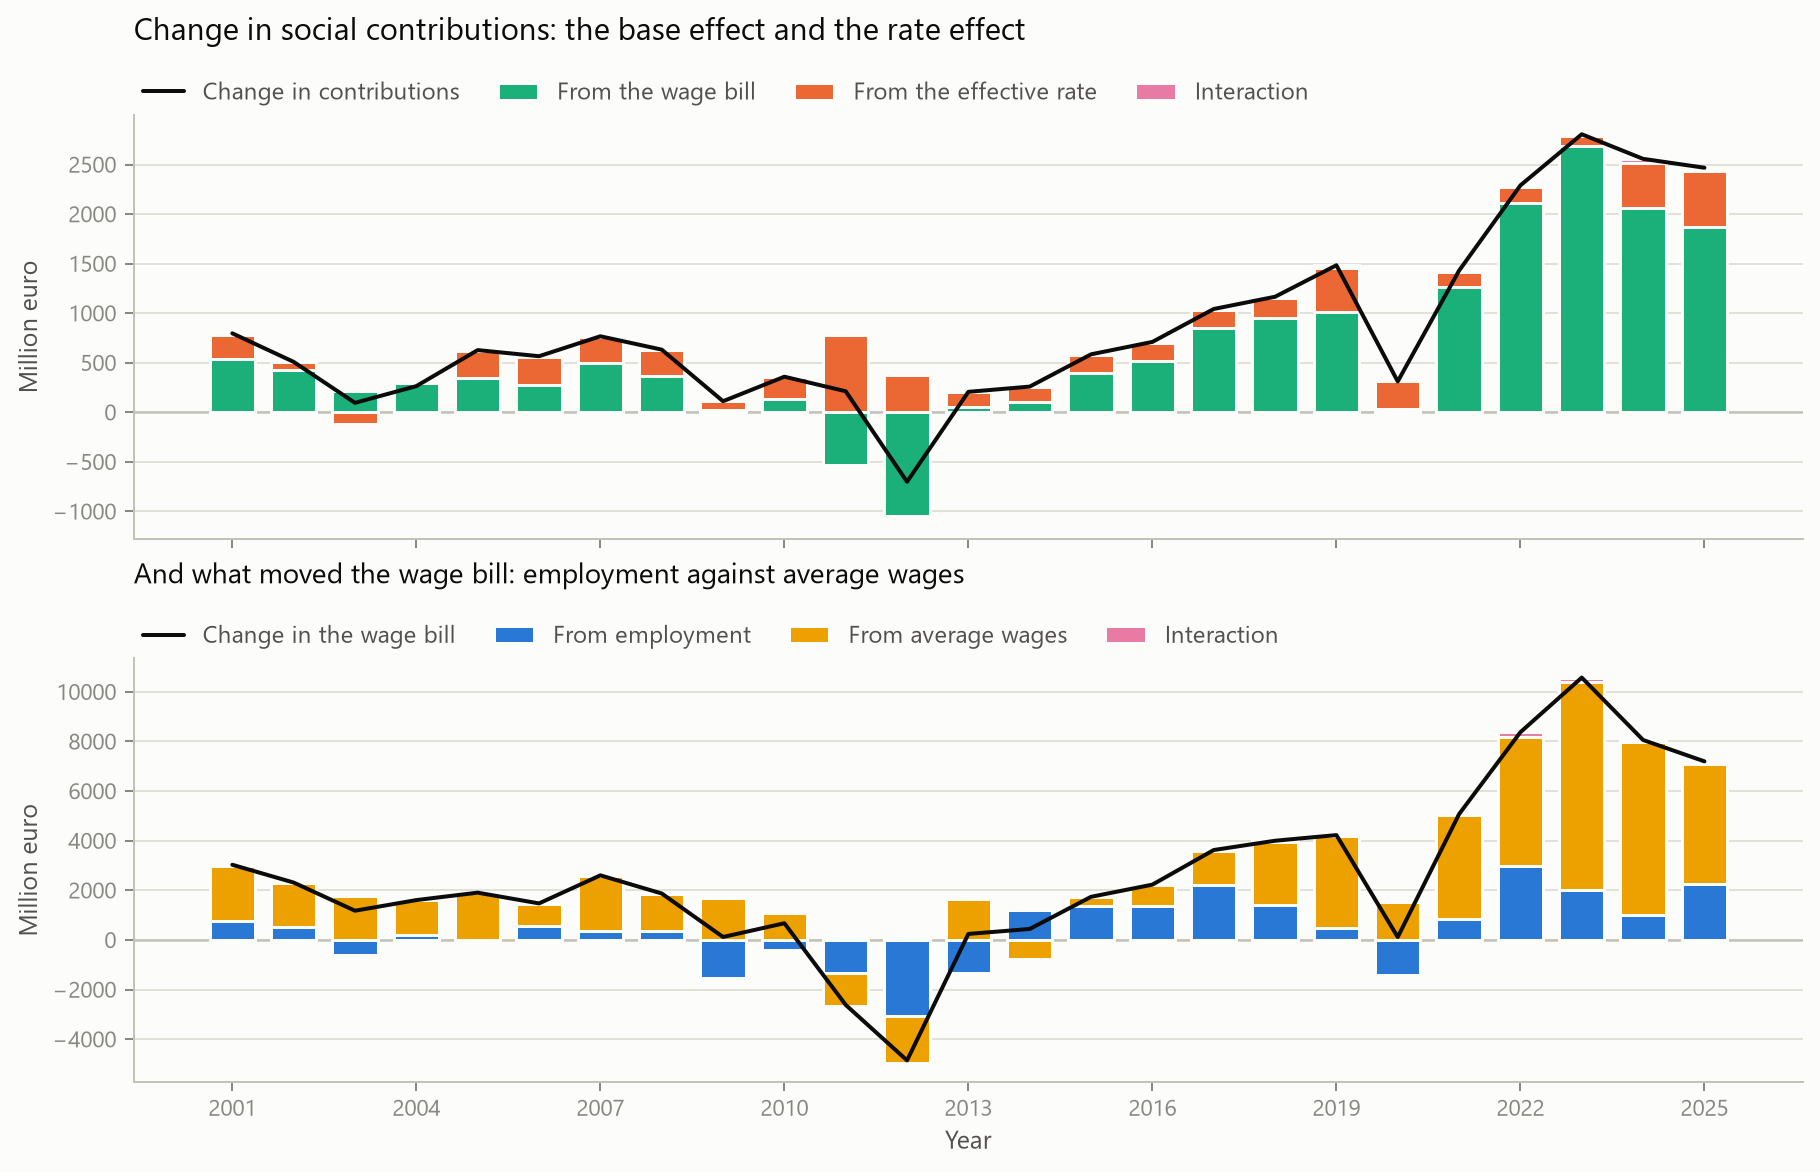
\includegraphics[width=\linewidth]{19_contribution_base.png}
\caption{Contributions and their base, 2001--\PanelEnd, in million euro. Upper panel: the
change in contributions split into a base effect and a rate effect. Lower panel: the
change in the wage bill split into employment and average wages. Both decompositions are
exact; the black line is the identity total in each.}
\label{fig:contributionbase}
\end{figure}

\subsection{A companion regression}

Section~\ref{sec:robustness} sets out why the nominal-GDP specification carries no weight,
and one of its faults was that the regressor was an aggregate that merely correlates with
the balance rather than the base a levy falls on. That fault is repairable, and repairing
it is the point of this specification.

Regressing the annual change in contributions on the annual change in the wage bill over
\WageBillObservations\ adjacent-year pairs gives a slope of \WageBillSlope\ with a HAC
standard error of \WageBillSlopeSe\ and an $R^2$ of \WageBillRSquared. Three things are
worth noting about that.

The slope is close to the average contributions-to-wage-bill ratio of \EffectiveRateMean.
That is consistent with a comparatively stable ratio component over the sample, but it is
not implied by the identity: Equation~\eqref{eq:contributionbase} would deliver
$\beta = \bar{\tau}$ only if $\Delta\tau$ and the interaction term were uncorrelated with
$\Delta W$, which nothing here establishes. The agreement is therefore a descriptive fact
about this sample rather than an arithmetic necessity.

The fit is an order of magnitude tighter than the nominal-GDP regressions, whose $R^2$
values span 0.07 to 0.18. That difference is the substantive argument for the
specification, not a claim about its sophistication.

And no changes are computed across the 1995-to-2000 gap in subsector accounts. That
matters more than it sounds: bridging the gap treats a five-year movement as annual, and
doing so drives the slope to 0.13 and the $R^2$ to 0.40. A single contaminated
observation was enough to destroy the relationship.

\subsection{What this does and does not establish}

The decomposition of Equation~\eqref{eq:contributionbase} is exact and descriptive. It
partitions a recorded movement; it does not show that the wage bill produced it, and it
says nothing about why employment or wages moved. The regression quantifies a
co-movement between two first differences and claims no identification.

What it does establish is that the recent growth in Social Security contributions is
overwhelmingly a base phenomenon rather than a rate phenomenon, and that within the base
it has lately been driven more by wages per employee than by the number of employees.
That is a mechanism in the accounting sense: it names the quantity whose movement the
contributions followed. It is not a causal account of why that quantity moved.

% Authored. Tables and numbers come from generated/.

\section{A European Benchmark: Is This Composition Unusual?}
\label{sec:benchmark}

Everything to this point describes one country. It establishes how Portugal's
general-government balance is composed and how persistent that composition is; it
cannot establish whether the composition is unusual, because a single-country study
has no comparison set. That distinction matters for how the results should be read:
a subsector pattern that is common across Europe invites a different explanation from
one that is peculiar to Portugal.

ESA 2010 requires the same subsector breakdown from every reporter, so the comparison
is available \citep{eurostat_gov_main,ecb_gfs}. We take net lending and net borrowing
by subsector for 1995--\PanelEnd\ from Eurostat and repeat the domestic definitions on
it.

\subsection{Construction}

Three choices matter, and each is a place where a careless benchmark would mislead.

\textbf{The non-Social-Security aggregate must include state government.} Portugal has
no S.1312 tier, so its aggregate is central plus local. Germany, Spain, Austria,
Belgium and Switzerland do have one, and omitting it would leave their identity open
and understate their non-Social-Security deficits. We therefore define
$\Bnonssf_{c,t} = B^{S.1311}_{c,t} + B^{S.1312}_{c,t} + B^{S.1313}_{c,t}$, treating a
missing state tier as contributing nothing because the tier does not exist rather than
because a value is unknown. With that definition the identity closes to published
rounding for every reporter.

\textbf{Ratios are computed in national currency.} Eurostat publishes shares of GDP to
one decimal, which is an unusable denominator for a ratio: a non-Social-Security
balance printed as $-0.2$ could lie anywhere in a band wide enough to move the offset
ratio by a quarter of its value. The levels carry far more precision, and the ratio is
currency-invariant. We additionally require the denominator to be at least $0.5$\% of
GDP in absolute size before reporting a ratio, so that a near-zero denominator cannot
manufacture a large one.

\textbf{Coverage is made comparable.} A country-year enters only if the four required
sectors --- the aggregate, central government, local government and social security funds
--- are all reported. The state tier is required conditionally rather than absolutely: a
country that reports S.1312 anywhere in its record must report it in that year too, while
a country that never reports it, Portugal among them, is not excluded for lacking a tier
it does not have. Requiring the tier unconditionally would drop every unitary reporter;
not requiring it at all would admit federal country-years whose non-Social-Security
aggregate is incomplete, and it is exactly those years in which the identity would fail
to close. A reporter then enters the summary only with at least fifteen complete years,
because a frequency computed over a handful of years is not comparable with one computed
over thirty. This leaves \BenchmarkCountries\ reporters over
\BenchmarkStart--\BenchmarkEnd, with Portugal contributing \BenchmarkYears\ years.

Two remarks on what the comparison is worth. Eurostat's Portuguese rows agree with our
domestic panel to rounding, which is an independent check on the extraction of
Section~\ref{sec:data} as well as the basis for the comparison. And this is a
distribution, not a test: locating Portugal within a spread of accounting compositions
says how common that composition is, not why any country's takes the form it does.

\subsection{Where Portugal sits}

Table~\ref{tab:benchmark} reports the composition for every reporter and
Table~\ref{tab:benchmarkposition} locates Portugal in each distribution.

\begin{table}[htbp]
\centering
\caption{Subsector composition across reporters, ordered by the frequency of a Social Security surplus. Sign frequencies are shares of the years each reporter covers completely.}
\label{tab:benchmark}
\small
\fitwidth{%
\begin{tabular}{@{}lrrrrrrr@{}}
\toprule
Reporter & N & Central $<0$ & SSF $>0$ & Mean SSF (\% GDP) & Surplus years & of which non-SSF $<0$ & Median offset \\
\midrule
FI & 31 & 0.774 & 1.000 & 2.45 & 11 & 6 & 0.540 \\
LU & 31 & 0.645 & 1.000 & 1.65 & 24 & 10 & 0.892 \\
DK & 31 & 0.355 & 0.935 & 0.05 & 21 & 0 & 0.008 \\
CY & 31 & 0.806 & 0.935 & 2.23 & 9 & 4 & 0.446 \\
PT & 31 & 1.000 & 0.935 & 0.71 & 4 & 4 & 0.141 \\
IT & 31 & 1.000 & 0.839 & 0.18 & 0 & 0 & 0.064 \\
EL & 31 & 0.903 & 0.839 & 0.97 & 6 & 3 & 0.206 \\
EE & 31 & 0.613 & 0.839 & 0.25 & 12 & 2 & 0.306 \\
IS & 28 & 0.536 & 0.821 & 0.16 & 10 & 0 & 0.043 \\
SE & 31 & 0.581 & 0.806 & 0.19 & 14 & 2 & 0.225 \\
SK & 31 & 1.000 & 0.742 & 0.42 & 0 & 0 & 0.061 \\
BG & 31 & 0.613 & 0.710 & 0.17 & 13 & 2 & 0.095 \\
RO & 31 & 1.000 & 0.710 & 0.13 & 0 & 0 & 0.084 \\
CH & 30 & 0.533 & 0.700 & 0.16 & 17 & 5 & 0.058 \\
LV & 31 & 0.968 & 0.677 & 0.35 & 2 & 0 & 0.316 \\
LT & 31 & 1.000 & 0.613 & 0.25 & 4 & 3 & 0.419 \\
DE & 31 & 0.774 & 0.613 & 0.04 & 8 & 2 & 0.085 \\
NL & 31 & 0.806 & 0.581 & 0.17 & 8 & 4 & 0.310 \\
IE & 31 & 0.516 & 0.581 & 0.09 & 16 & 3 & 0.167 \\
BE & 31 & 1.000 & 0.581 & 0.06 & 3 & 2 & 0.072 \\
AT & 31 & 0.968 & 0.548 & 0.02 & 2 & 0 & 0.056 \\
HU & 31 & 1.000 & 0.548 & 0.02 & 0 & 0 & 0.045 \\
SI & 31 & 0.935 & 0.516 & -0.05 & 3 & 1 & 0.043 \\
PL & 31 & 1.000 & 0.484 & 0.24 & 0 & 0 & 0.263 \\
HR & 31 & 0.871 & 0.452 & -0.12 & 4 & 1 & 0.124 \\
FR & 31 & 1.000 & 0.419 & -0.20 & 0 & 0 & 0.072 \\
CZ & 31 & 0.935 & 0.387 & -0.04 & 4 & 0 & 0.051 \\
ES & 31 & 0.903 & 0.355 & -0.27 & 3 & 0 & 0.464 \\
\bottomrule
\end{tabular}%
}
\par\smallskip
\begin{minipage}{\linewidth}\footnotesize\itshape The non-Social-Security aggregate is central plus state plus local government, so federal reporters are treated consistently with unitary ones. Reporters with fewer than fifteen complete years are excluded, because a frequency over a handful of years is not comparable with one over thirty.\end{minipage}
\end{table}

\begin{table}[htbp]
\centering
\caption{Portugal's position in each cross-country distribution. The percentile is the share of reporters below Portugal's value.}
\label{tab:benchmarkposition}
\small
\fitwidth{%
\begin{tabular}{@{}lrrrrr@{}}
\toprule
Metric & Portugal & Cross-country median & Minimum & Maximum & Percentile \\
\midrule
Share of years with a Central Government deficit & 1.000 & 0.903 & 0.355 & 1.000 & 68 \\
Share of years with a Social Security surplus & 0.935 & 0.689 & 0.355 & 1.000 & 82 \\
Share of years with an aggregate surplus & 0.129 & 0.129 & 0.000 & 0.774 & 39 \\
Mean Social Security balance (\% GDP) & 0.706 & 0.168 & -0.271 & 2.448 & 82 \\
Median offset ratio, where defined & 0.141 & 0.110 & 0.008 & 0.892 & 54 \\
\bottomrule
\end{tabular}%
}
\end{table}


The answer is not uniform across the paper's findings, and that is the substantive
result of this section.

\paragraph{The Central Government deficit is not unusual.} Portugal records a Central
Government deficit in \PtCentralNegativeShare\% of its reported years, which places it
at the \PtCentralPercentile th percentile --- but \CentralAlwaysNegativeCountries\ of
the \BenchmarkCountries\ reporters also record one in every single year. A persistently
deficit-running central tier is a common European pattern, not a Portuguese
peculiarity. Read on its own, the domestic finding that Central Government is negative
in all \CentralNegativeYears\ years would invite the opposite impression.

\paragraph{The Social Security surplus is unusual, in both frequency and size.}
Portugal records a Social Security surplus in \PtSsfPositiveShare\% of years against a
cross-country median of \PtSsfShareMedian\%, at the \PtSsfSharePercentile th
percentile. Its mean Social Security balance is \PtSsfMeanPct\% of GDP against a median
of \PtSsfMeanMedian\%, again at the \PtSsfMeanPercentile th percentile. On both
measures Portugal sits in the upper tail.

\paragraph{The typical offset magnitude is ordinary.} Portugal's median offset ratio,
over the years in which it is defined, is \PtOffsetMedian\ against a cross-country
median of \OffsetMedianAcrossCountries, at the \PtOffsetPercentile th percentile. In a
typical year the Portuguese Social Security surplus offsets no more of the
non-Social-Security deficit than elsewhere. What distinguishes Portugal is the recent
years, in which the ratio exceeds one, not the central tendency.

That conclusion rests on the denominator floor, which is a choice rather than a property
of the data, so it is worth checking whether the conclusion survives other choices.
Sweeping the floor from \OffsetFloorLow\ to \OffsetFloorHigh\ percent of GDP moves
Portugal's percentile only between \OffsetPercentileLow\ and \OffsetPercentileHigh: the
position stays near the middle of the distribution throughout. Had the percentile moved
sharply with the floor, the finding would have been an artefact of where we set it.

\begin{figure}[htbp]
\centering
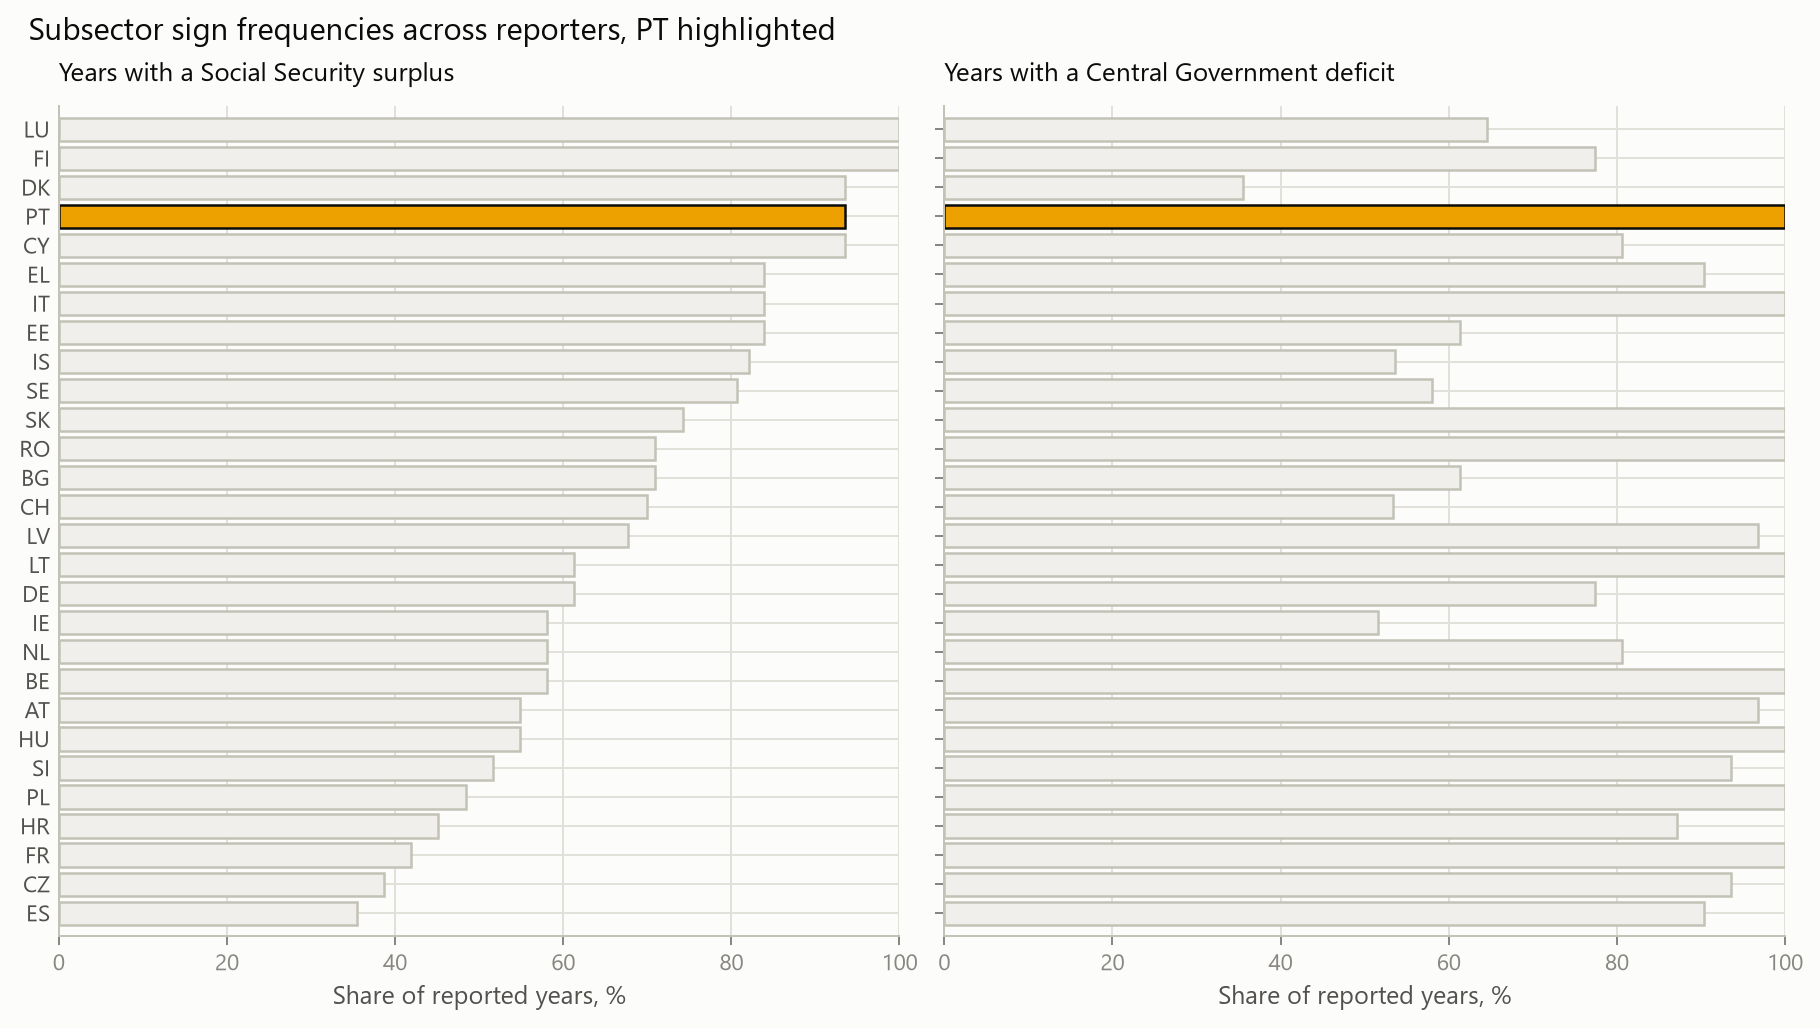
\includegraphics[width=\linewidth]{17_european_benchmark.png}
\caption{Subsector sign frequencies across reporters, Portugal highlighted, ordered by
the frequency of a Social Security surplus. Left: share of reported years with a Social
Security surplus. Right: share with a Central Government deficit. Portugal is in the
upper tail of the first and shares the maximum of the second with several reporters.}
\label{fig:benchmark}
\end{figure}

\begin{figure}[htbp]
\centering
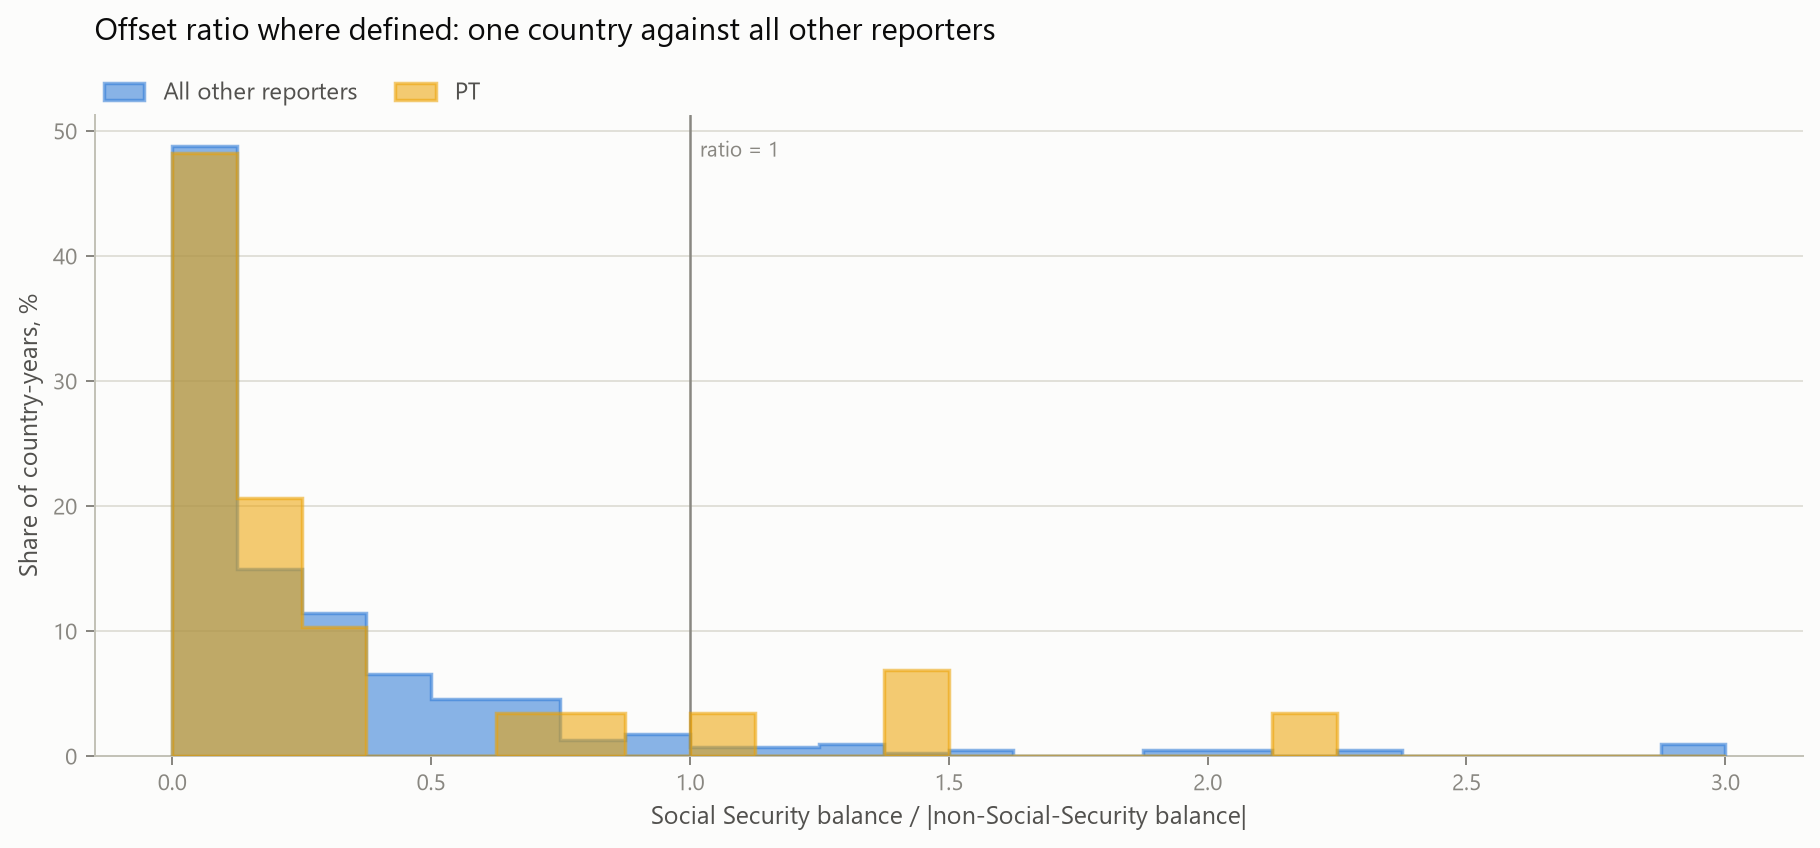
\includegraphics[width=\linewidth]{18_european_offset_distribution.png}
\caption{Offset ratio where defined: Portugal against all other reporters pooled, as a
share of each group's defined country-years. Values above three are clipped to the last
bin. The Portuguese distribution is not shifted relative to the others; its recent years
sit in the right tail of both.}
\label{fig:offsetdistribution}
\end{figure}

\subsection{The composition of a surplus year}

The sharpest comparison is not a sign frequency but the structure of the surplus years
themselves, because that is the paper's headline composition restated as a
cross-country question: when a country records an aggregate surplus, is its
non-Social-Security balance in deficit?

Across the \CountriesWithSurplus\ reporters with at least one aggregate surplus, that
composition holds in \SurplusYearsOffsetting\ of \SurplusYearsTotal\ surplus
country-years, or \SurplusOffsettingShare\%. It is therefore a minority pattern: most
European surpluses are recorded with the non-Social-Security tiers also in surplus, or
close to balance.

Portugal is the exception in the strict sense. Of the \CountriesWithSurplus\ reporters,
\CountriesAllOffsetting\ record a negative non-Social-Security balance in \emph{every}
one of their aggregate-surplus years, and Portugal is among them, at
\PtSurplusOffsetting\ of \PtSurplusYears.

The pooled figure weights by country-year, so a reporter with two dozen surplus years
counts for more than one with three. Weighting by country instead asks a different and
equally reasonable question --- of a country's own surplus years, what share pair with a
negative non-Social-Security balance? --- and the two agree: the country-weighted median
is \SurplusCountryMedian\%, with quartiles at \SurplusCountryLowerQuartile\% and
\SurplusCountryUpperQuartile\%, against the pooled \SurplusOffsettingShare\%. Portugal
sits at the \SurplusCountryPercentile th percentile of that distribution. Because the two
weightings can disagree and neither is obviously correct, both are reported.

That result needs its sample stated plainly alongside it. Portugal has only
\PtSurplusYears\ surplus years, so ``all of them'' is four observations, and several
reporters with more surplus years have high but not unanimous shares. The defensible
statement is therefore the conjunction: the composition is a minority pattern in Europe,
Portugal exhibits it in every surplus year it has recorded, and the number of such years
is small. We would not read a stronger claim than that from
\PtSurplusYears\ observations.

\subsection{What the benchmark changes}

It changes the reading of two results and confirms a third.

The Central Government finding is weaker than it looks in isolation: a permanently
deficit-running central tier is normal in Europe. The Social Security finding is
stronger: both the frequency and the size of the Portuguese surplus sit in the upper
tail. And the composition of the surplus years is genuinely distinctive, subject to the
sample caveat above.

None of this identifies a cause. Countries differ in how they assign contributory
schemes between tiers, in whether they operate a state-government level, in the maturity
of their pension systems and in how they route transfers between subsectors --- and the
benchmark holds none of that constant. It establishes that the Portuguese composition is
unusual in a specific, stated respect, which is what the rest of the paper could not do.

% Authored. Numbers come from generated/macros.tex.

\section{Conclusion}
\label{sec:conclusion}

Portugal's general-government balance, decomposed across institutional subsectors
over \PanelYears\ years, has a composition that is asymmetric and remarkably stable.
The Central Government balance is negative in every one of the
\CentralNegativeYears\ observations. The Social Security balance is positive in
\SsfPositiveYears, with a longest unbroken run of \SsfLongestPositiveRun\ years.
Regional and Local Government is the only subsector that changes sign with any
regularity, and it is small in both directions. The aggregate tracks Central
Government closely inside each statistical regime, correlating at
\HistoricalTrackingCorrelation\ before the 1995 splice and \ModernTrackingCorrelation\
after it. The aggregate is positive
in \NumPositiveYears\ years, and in each of them the combined non-Social-Security
balance is negative --- from which, given the identity, the rest of that year's
composition follows.

Against \BenchmarkCountries\ European reporters, the composition is distinctive in one
specific respect and unremarkable in another. A permanently deficit-running central
tier is common, so the Central Government finding is weaker than it appears in
isolation. The Social Security surplus sits in the upper tail on both frequency and
size. And Portugal is the only reporter whose every aggregate-surplus year combines
that surplus with a negative non-Social-Security balance --- a composition present in
\SurplusOffsettingShare\% of European surplus years, though Portugal's own count is
only \PtSurplusYears.

On the Social Security side, most of the recent increase in contributions is
algebraically associated with growth in the aggregate employee wage bill rather than with
movement in the contributions-to-wage-bill ratio. Of the \BaseContributionsChange\ million
euro rise in \BaseYear,
\[
\BaseContributionsChange = \BaseFromWageBill + \BaseFromRatio + \BaseRatioInteraction,
\]
the three terms being the wage-bill component, the ratio component and their interaction.
The wage bill itself rose by \BaseWageBillChange\ million over the same year, and that is
a second and separate identity:
\[
\BaseWageBillChange = \BaseFromEmployment + \BaseFromAverageWage + \BaseWageInteraction,
\]
in employees, average wage and interaction. The two share a factor but not a total, and
the terms of the second are components of $\Delta W$ rather than parts of the
\BaseFromWageBill\ million wage-bill component of the first. Read together they say that
the movement was predominantly in the reference base rather than in the ratio, and that
within the base it came more from wages per employee than from employee numbers. That is
a mechanism in the accounting sense --- it names the quantity the contributions followed
--- and not a causal account of why that quantity moved.

Two results cut against readings that the aggregate series invites.

The first concerns Central Government. Its balance is negative throughout the panel,
but its primary balance is positive in \PrimaryPositiveYears\ of the
\PrimaryObservedYears\ years for which detailed accounts exist ---
\HistoricalPrimaryPositive\ of \HistoricalPrimaryYears\ before the 1995 splice and
\ModernPrimaryPositive\ of \ModernPrimaryYears\ after it, so the positive years are if
anything a historical phenomenon rather than a recent one. A persistently negative B.9
does not imply a persistently negative primary balance, and interest is the arithmetic
that separates them: it averaged \HistoricalInterestMean\% of GDP in the historical
regime against \ModernInterestMean\% in the modern one.

The second concerns Social Security. The ESA 2010 Social Security Funds sector and
the CFP budget-execution systems are different accounting objects whose balances
differ in every one of the \SsfBoundaryYears\ years they overlap, by between
\SsfBoundaryMin\ and \SsfBoundaryMax\ million euro. Quoting one where the other
belongs introduces an error of that order with no signal that it has occurred.

\subsection{What this paper does not establish}

The decomposition is an accounting identity. It reallocates a recorded quantity and
estimates nothing, and three inferences do not follow from it.

It does not license a counterfactual. That a positive Social Security balance exceeds
a negative non-Social-Security balance in a given year says those two published
numbers stand in a particular ratio. It says nothing about what the aggregate would
have been under a different institutional arrangement, because that counterfactual
would move contribution rates, entitlements and transfers together and the identity
models none of them.

It does not attribute responsibility. A subsector accounting arithmetically for most
of a movement has not been shown to have produced it.

It does not speak to sustainability. Neither the headline nor the primary balance
determines the debt path, which also depends on stock-flow adjustments that are the
larger term in several years of these data.

It does not explain why Portugal's composition differs. The benchmark establishes that
it does, in a stated respect, while holding no institutional feature constant.

Two further limits are properties of the data rather than of the method. Magnitudes
are regime-specific and cannot be pooled across the 1995 splice; the pooled aggregate
mean of \GgMeanPooled\% of GDP describes neither the \GgMeanHistorical\% of
\PanelStart--1994 nor the \GgMeanModern\% of 1995--\PanelEnd. And
\ProvisionalYears\ are provisional at source: they are the years discussed in most
detail here and the years most likely to be restated by a later vintage.

\subsection{Extensions}

Two extensions follow naturally.

The contribution base of Section~\ref{sec:contributionbase} stops at the aggregate wage
bill. Splitting it by sector, contract type or earnings band would say which part of the
base carried the growth, and the same identity would apply unchanged; the data required
are published but are not in the bundle assembled here.

Extending the benchmark of Section~\ref{sec:benchmark} would sharpen it. It currently
compares compositions while holding nothing else constant, so it cannot separate a
Portuguese peculiarity from the consequence of an institutional choice made elsewhere:
whether a country operates a state-government tier, how it assigns contributory schemes
between tiers, how mature its pension system is, and how it routes transfers between
subsectors. Conditioning on those would turn a distribution into a comparison.


\bibliographystyle{plainnat}
\bibliography{references}

\appendix
% Authored. Numbers come from generated/macros.tex.

\section{Change-Point Sensitivity in Full}
\label{sec:changepoints}

Section~\ref{sec:robustness} summarises the sensitivity of the piecewise-constant
mean shifts. This appendix records the specification and the full grid, so the
summary can be checked rather than taken.

\subsection{Specification}

For a balance ratio $y_1,\dots,y_n$ inside one statistical regime, the model
partitions the index range into $k+1$ contiguous segments and fits a constant to
each. The partition minimises total within-segment squared error,
\[
\min_{0 = b_0 < b_1 < \cdots < b_k < b_{k+1} = n}
\ \sum_{j=0}^{k} \sum_{t = b_j + 1}^{b_{j+1}} \left(y_t - \bar{y}_{[b_j, b_{j+1}]}\right)^2,
\]
solved exactly by dynamic programming rather than by a greedy or binary-segmentation
heuristic. Selection over $k$ uses
\[
\mathrm{BIC}(k) = n \log\!\left(\frac{\mathrm{RSS}(k)}{n}\right) + (2k+1)\log n,
\]
where the parameter count $2k+1$ charges for $k+1$ segment means and $k$ break
locations. Charging for the locations is the conservative choice: it penalises an
additional break twice and makes the model less willing to claim one. Zero breaks is
always admissible.

Two tuning parameters are not estimated: the minimum segment length and the maximum
number of breaks. The baseline sets them to five years and two breaks per regime.

\subsection{The grid}

Detection is re-run over the product of

\[
\text{minimum segment} \in \{4, 5, 6, 7\}
\quad \text{and} \quad
\text{maximum breaks} \in \{1, 2, 3\},
\]

giving \BreakSpecifications\ specifications for each of the \BreakSeries\
regime-subsector series. Three quantities are persisted for each series: the modal
number of breaks and the share of the grid selecting it, the modal set of dates and
the share of the grid returning exactly that set, and the number of distinct date
sets the grid produced.

The last of these is the most informative single number. A series whose grid returns
one date set is telling us something about the series; a series whose grid returns
six is telling us about the tuning parameters.

\subsection{Reading the result}

\BreakModalAgree\ of \BreakSeries\ series have a preferred specification that agrees
with the modal grid outcome. Where the two disagree, the modal column is the more
reliable summary and the preferred date should not be quoted alone. The least stable
series is \WeakestBreakSector\ in the modern regime, at
\WeakestBreakShare\% modal agreement across \WeakestBreakSets\ distinct date sets.

Two further limits apply regardless of the grid. A minimum segment length of five
years means a shift within the last four years of the sample is undetectable by
construction. And selecting a mean shift does not imply the series is
piecewise-constant; it is the best fit inside a restricted model class, chosen
because the sample is too short to support a richer one.

The full per-specification grid, the BIC ladder over admissible break counts and the
stability summary are persisted as
\path{outputs/tables/structural_break_sensitivity.csv},
\path{outputs/tables/structural_break_bic_ladder.csv} and
\path{outputs/tables/structural_break_stability.csv}.

% Authored. Numbers come from generated/macros.tex.

\section{Data and Code Availability}
\label{sec:reproducibility}

\subsection{What is archived}

The accompanying repository retains the raw source workbooks as downloaded, a
SHA-256 digest of each, the source-specific intermediate extractions, the canonical
processed panels, every calculated analysis table, the figures, and the executed
notebooks with their outputs stored in place. No stage of the chain from a published
workbook to a number in this paper is missing.

\subsection{How this paper relates to the technical report}

The repository contains two documents and they have different jobs.

The technical report is generated end to end: its prose is a thin restatement of the
persisted artefacts, it carries every analysis the pipeline computes, and no part of
it is authored by hand. It is the place to look for material this paper omits ---
the fixed-capital-formation diagnostic, the debt and stock-flow reconciliation, the
full transition matrices, the intergovernmental-transfer sensitivity and the
descriptive macroeconomic co-movement.

This paper is authored. Its argument, its structure and its prose are written, and
it carries only the evidence that argument needs.

What the two share is the arithmetic. Every table in this paper is written by the
pipeline from a persisted artefact, and every number in its prose is a LaTeX macro
generated from one. A sentence here cannot hold a value the data no longer support:
if an artefact changes, the macro changes with it, and a macro that ceases to exist
fails the build rather than rendering silently as nothing. The authored text lives in
\path{paper/sections/}; the generated inputs live in \path{paper/generated/} and are
never edited by hand.

\subsection{Reproduction}

\begin{verbatim}
poetry install
make all          # pipeline, notebooks, tests
make paper        # this document
\end{verbatim}

The pipeline is deterministic: the same bundled inputs produce the same outputs, and
the outputs are committed, so a reader can check a number without running anything.

\subsection{Known limitations of the archive}

The bundled sources are a single vintage. \ProvisionalYears\ are provisional at
source and a later vintage will restate them; reproducing this paper against newer
files will therefore reproduce the method but not necessarily every figure. The
vintage of each retained file is recorded in Table~\ref{tab:sources} for that reason.

The \GapYears\ missing years of subsector detailed accounts, 1996--1999, are absent
from both source families. They are not imputed here and cannot be recovered from the
bundled data.


\end{document}
